% !TEX root = ../YourName-Dissertation.tex
\chapter[Beamline Characterization of Diffraction Efficiency]{Beamline Characterization of \\Diffraction Efficiency}\label{ch:diff_eff} 
%\chapter[Characterization of Diffraction Efficiency for X-ray Reflection Gratings]{Characterization of Diffraction \\Efficiency for X-ray Reflection \\Gratings}\label{ch:diff_eff} 
%%%%%%%%%%%%%%%%%%%%%%%%%%%%%%%%%%%%%%%%%--------------------------------------------------
Blazed reflection gratings are motivated in \cref{ch:introduction} as a technology suitable for the \emph{XGS} of the \emph{Lynx X-ray Observatory} \cite{Lynx_web,Gaskin19}, which has a main scientific objective of measuring the diffuse, highly-ionized baryonic content in extended galactic halos and the intergalactic medium through absorption spectroscopy of active galactic nuclei [\emph{cf.\@} \cref{sec:astro_plasmas}]. 
Described in \cref{sec:grating_tech_intro}, such a spectrometer uses many identical gratings aligned into modular arrays that each intercept radiation in an \emph{extreme off-plane mount}, where the cone half-opening angle, $\gamma$, is on the order of a degree while the azimuthal incidence angle, $\alpha$, is free to match the blaze angle, $\delta$, in a \emph{Littrow configuration}, where the azimuthal diffracted angle associated with the grating blaze is $\beta = \alpha = \delta$ [\emph{cf.\@} \cref{fig:conical_reflection_edit}]. 
With the research presented in \cref{ch:master_fab,ch:grating_replication} utilizing diffraction-efficiency testing as a means for characterizing the performance of fabricated x-ray reflection gratings [\emph{cf.\@} \cref{sec:ch1_conclusions}], this chapter outlines the relevant beamline methodology in \cref{sec:als_testing} following an established test procedure intended for the extreme off-plane geometry \cite{Miles18}. 
Additionally, \cref{sec:integral_method} describes how, with the aid of the \textsc{PCGrate-SX} software package (\textsc{I.\ I.\ G., Inc.\@}) \cite{PCGrate_web}, measured diffraction-efficiency data can be modeled using the \emph{integral method} to solve the Helmholtz equation for a periodic surface-relief boundary that represents the interface between vacuum and a reflection grating. 
A summary of these methods for characterizing soft x-ray diffraction efficiency is then provided in \cref{sec:ch2_summary}.\footnote{The beamline experimentation described in \cref{sec:als_testing} and utilized in \cref{ch:master_fab,ch:grating_replication} was carried out under an ALS general user proposal agreement lasting through 2017 and 2018.} 

\section[Reflection Grating Testing at the Advanced Light Source]{Reflection Grating Testing at the ALS}\label{sec:als_testing}
%%%%%%%%%%%%%%%%%%%%%%%%%%%%%%%%%%%%%%%%%--------------------------------------------------
Beamline 6.3.2 of the Advanced Light Source (ALS) \cite{ALS_web,ALS_632} at Lawrence-Berkeley National Laboratory \cite{LBNL_web} provides a test station for extreme ultraviolet (EUV) and soft x-ray reflectometry where, under high vacuum, highly-coherent, monochromatic radiation tunable across $\SI{40}{\nm} \gtrapprox \lambda \gtrapprox \SI{1}{\nm}$ strikes a stage-mounted optic while a movable photodiode detector is used to measure the intensity of ingoing and outgoing radiation \cite{Underwood96,Gullikson01}. 
For the physical reasons outlined in \cref{sec:SXR_med}, soft x-rays and EUV radiation are easily absorbed by carbon, nitrogen and oxygen atoms found in air molecules, and as a result, optical testing occurs under high vacuum with the aide of a graphical user interface that enables control of the beam wavelength, $\lambda$, in addition to optic-mount and detector motion. 
Using this facility, the specular reflectivity of a mirror [\emph{cf.\@} \cref{eq:fresnel_refl_def}]: 
\begin{equation}
 \mathcal{R} \left( \lambda \right) \equiv \frac{\mathcal{I}''\!\left( \lambda \right)}{\mathcal{I}_{\text{inc}} \!\left( \lambda \right)} ,
 \end{equation} 
can be experimentally determined for a given incidence angle by measuring the intensity of the reflected beam, $\mathcal{I}''\left( \lambda \right)$, relative to that of the incident beam, $\mathcal{I}_{\text{inc}} \!\left( \lambda \right)$. 
Similarly, the \emph{absolute diffraction efficiency} of a reflection grating, defined as the intensity ratio between the $n^{\text{th}}$ diffracted order and the unobstructed beam \cite{Loewen97}: %\cref{eq:scalar_efficiency}:
\begin{equation}\label{eq:diffraction_efficiency}
 \mathscr{E}_n \! \left( \lambda \right)  \equiv \frac{\mathcal{I}_n \! \left( \lambda \right)}{\mathcal{I}_{\text{inc}} \! \left( \lambda \right)} \quad \text{for } n = 0, \pm 1, \pm 2, \pm 3 \dotsc , 
 \end{equation} 
can also be measured using this beamline facility by comparing the intensity of each propagating order, $\mathcal{I}_n \! \left( \lambda \right)$, to $\mathcal{I}_{\text{inc}} \!\left( \lambda \right)$ for a particular grating geometry established using stage rotations inside the test chamber. 

A photograph of the chamber interior, which features an aperture for the monochromatic beam, detectors attached to goniometric staging and a central optic mount with linear and rotational degrees of freedom is shown in \cref{fig:beamline_photoA}, where the distance from the point of incidence on the optic mount to the detector staging (\emph{i.e.}, the \emph{throw}) is $L \approx \SI{235}{\mm}$.  
\begin{figure}
 \centering
 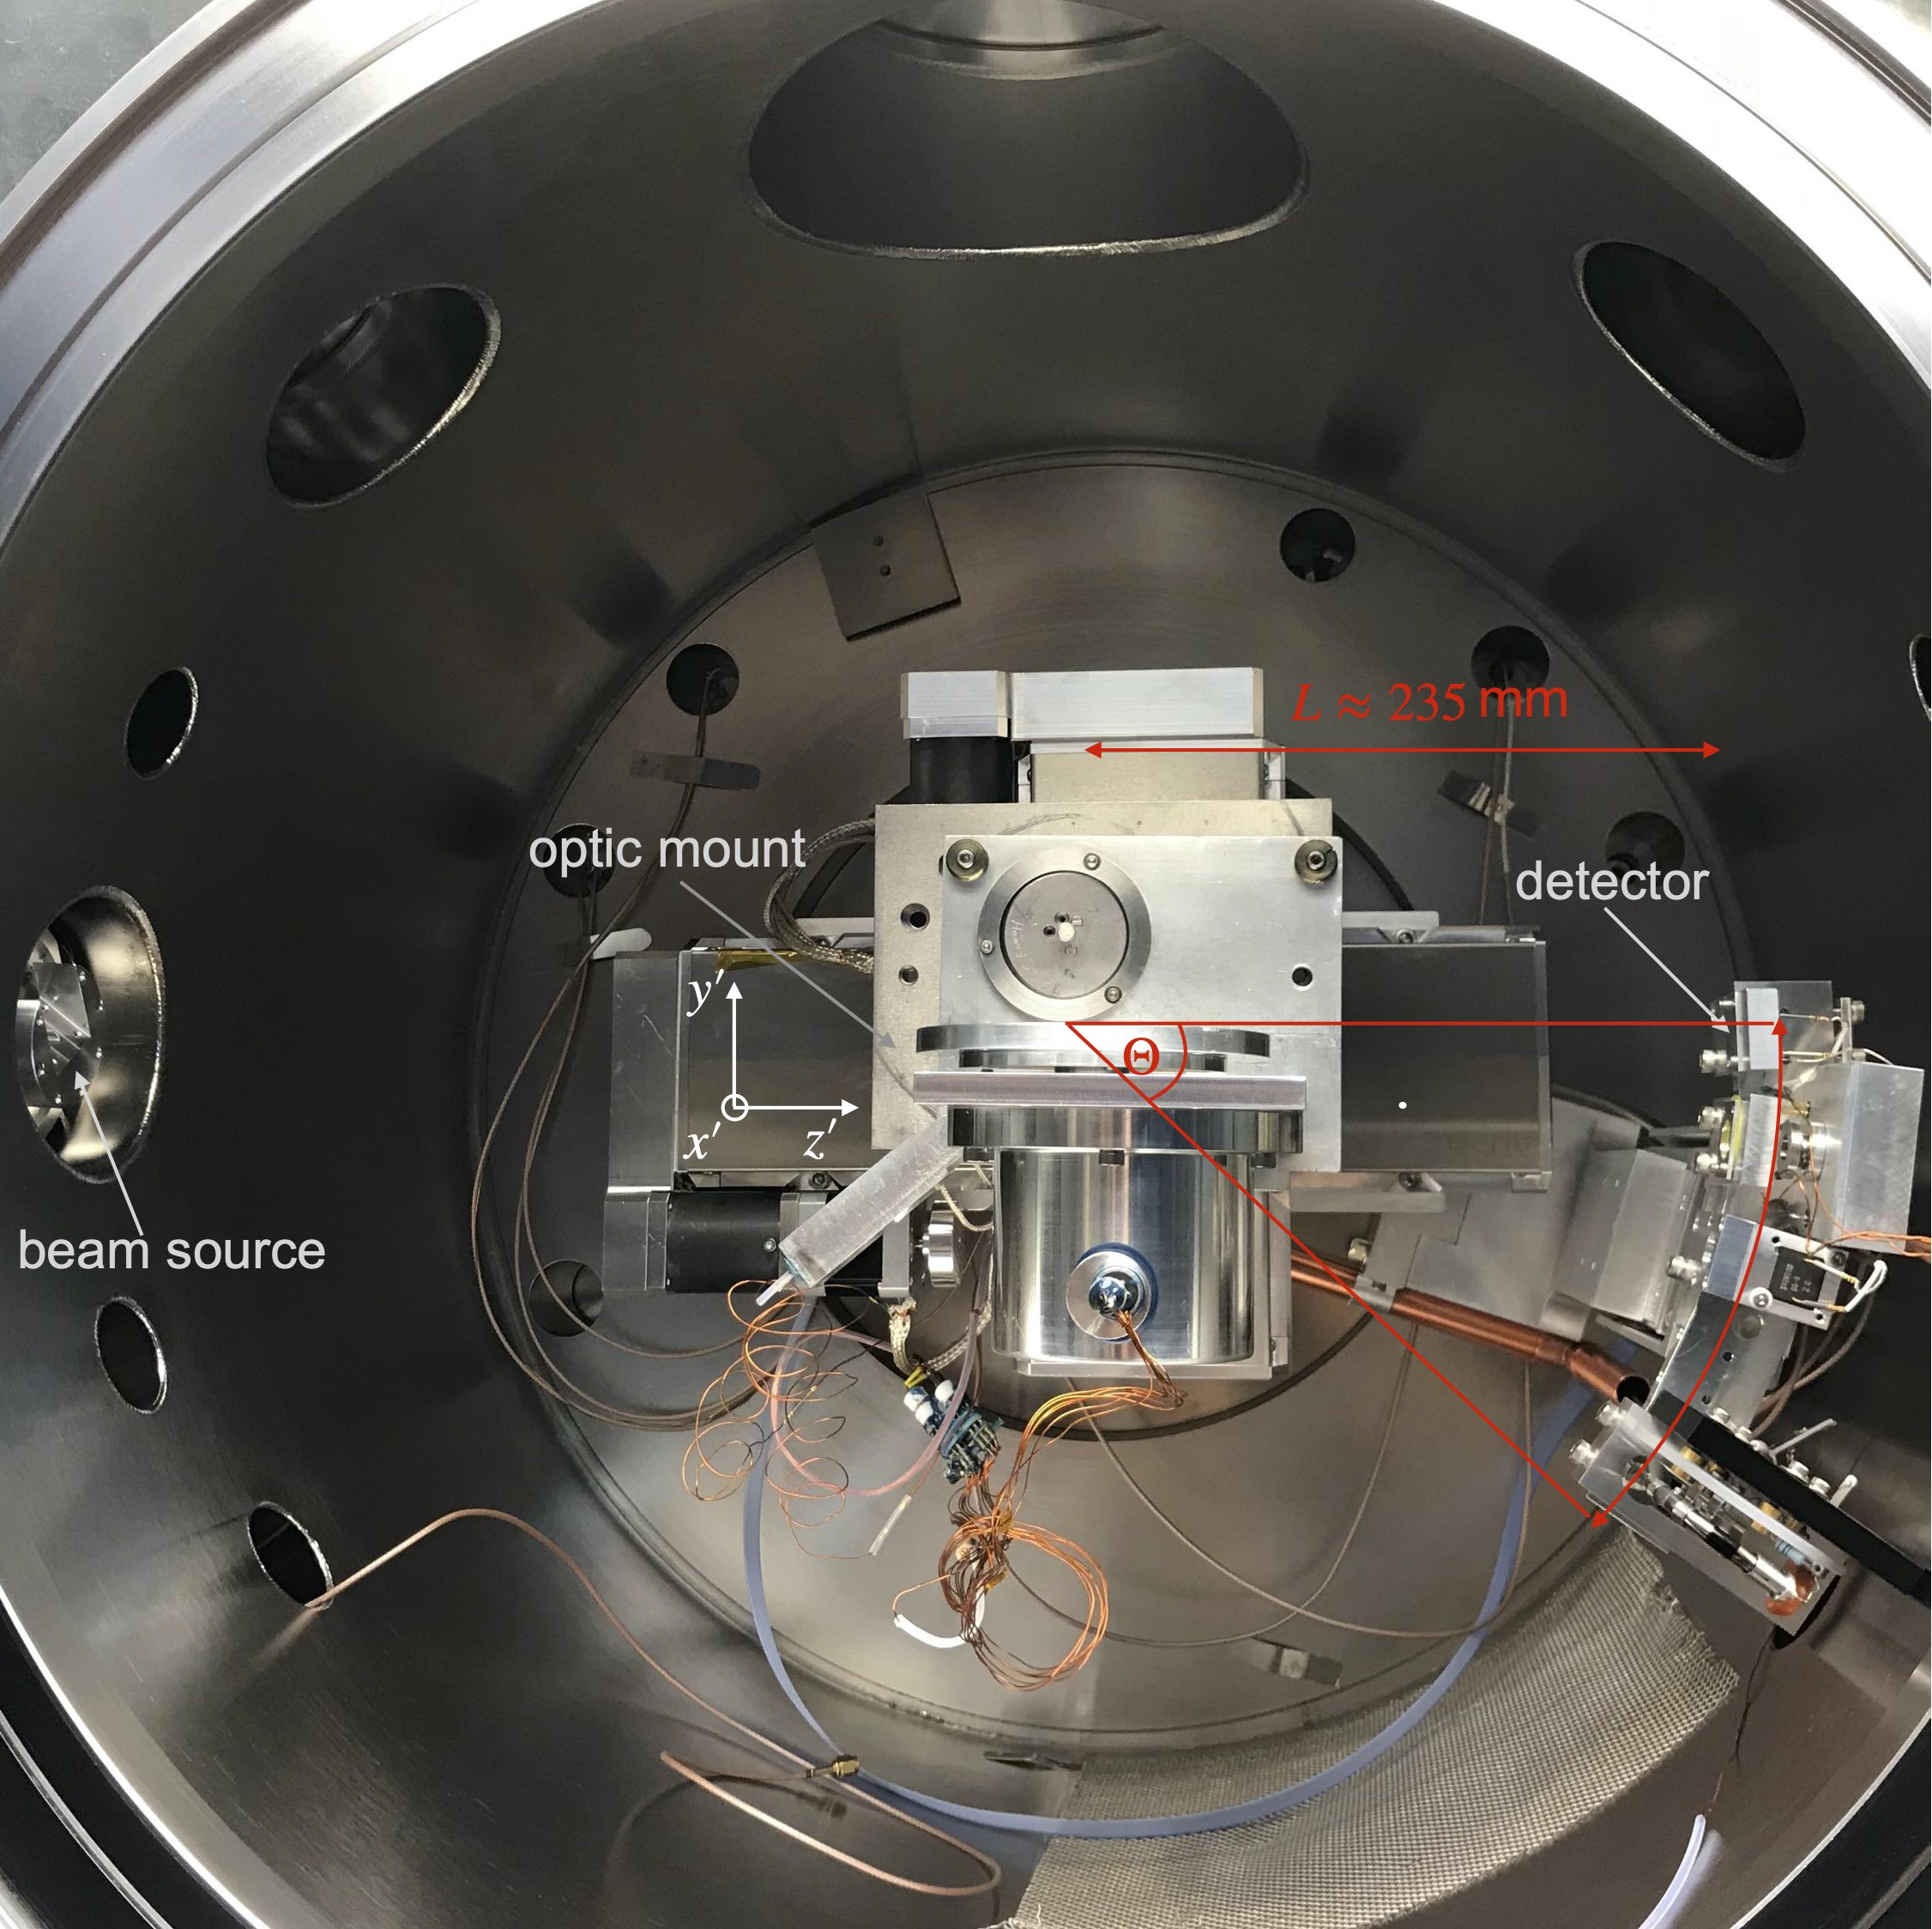
\includegraphics[scale=0.172]{Chapter-2/Figures/ALS_photoA.jpg}
 \caption[Overview of the station for soft x-ray reflectometry at beamline 6.3.2 of the Advanced Light Source (ALS)]{Beamline 6.3.2 of the ALS provides a station for EUV and soft x-ray reflectometry, where a highly-coherent beam produced by a monochromator travels along the $z'$-direction to a photodiode attached to controllable staging that, owing to the cylindrical shape of the vacuum chamber, can move linearly in the $x'$-direction and goniometrically in the $\Theta$-direction. A reflection grating is mounted on staging with translational and rotational degrees of freedom that can be moved to intercept the beam. This optic mount has rotational degrees of freedom that enable grating geometry to be set to a grazing-incidence, near-Littrow configuration.}\label{fig:beamline_photoA}
 \end{figure}
The detector staging can move linearly along the $x'$-direction and goniometrically about the $x'$-axis such that an angular position $\Theta$ maps to a vertical distance $y' \approx L \sin \left( \Theta \right)$, where any reference point can be used for $\Theta = 0$. 
As described in \cref{sec:grating_tech_intro} and illustrated in \cref{fig:conical_reflection_edit}, an extreme off-plane geometry causes a far-field diffraction pattern where propagating orders are confined to the surface of a cone with a half-opening angle, $\gamma$, of a few degrees; the locations of these orders are described by the \emph{generalized grating equation} \cite[\emph{cf.\@} \cref{eq:off-plane_orders,eq:off-plane_incidence_orders}]{Loewen97}: 
\begin{equation}\label{eq:off-plane_orders_ch2}
 \sin \left( \alpha \right) + \sin \left( \beta \right) = \frac{n \lambda}{d \sin \left( \gamma \right)} \quad \text{for } n = 0, \pm 1, \pm 2, \pm 3 \dotsc ,
 \end{equation}
with $d$ as the groove spacing, $\alpha$ as the azimuthal incidence angle and $\beta$ as the azimuthal diffracted angle of the $n^{\text{th}}$ order. 
Therefore, $\mathscr{E}_n \! \left( \lambda \right)$ can be determined according to \cref{eq:diffraction_efficiency} by sampling the diffracted arc as a function of $x'$ and $y'$ to measure $\mathcal{I}_n \! \left( \lambda \right)$ for each propagating order. 

Before $\mathscr{E}_n \! \left( \lambda \right)$ can be measured across a range wavelengths, a series of steps must be carried out to establish a desired grating geometry with specified values for $\alpha$ and $\gamma$. 
The condition for \emph{total external reflection (TER)} [\emph{cf.\@} \cref{sec:planar_interface}] requires that the groove-facet incidence angle for a grating with a blaze angle $\delta$, given by \cref{eq:angle_on_groove}, be smaller than the \emph{critical angle}, $\zeta_c (\omega)$ [\emph{cf.\@} \cref{eq:critical_angle}]: 
\begin{equation}\label{eq:TER_condition_grat}
 \zeta \equiv \arcsin \left[ \sin \left( \gamma \right) \cos \left( \delta - \alpha \right) \right] < \zeta_c (\omega) \approx \sqrt{2 \delta_{\nu} (\omega)} 
 \end{equation} 
with $\tilde{\nu}(\omega) \equiv 1 - \delta_{\nu} (\omega) + i \xi(\omega)$ as the complex index of refraction for given material [\emph{cf.\@} \cref{sec:x-ray_index}]. 
Moreover, \cref{sec:grating_tech_intro} motivates the use of the Littrow configuration with $\alpha = \beta = \delta$ and $\zeta = \gamma$. 
In practice, however, a \emph{near-Littrow} configuration with $\alpha \approx \delta$ and $\zeta \lessapprox \gamma$ is realized for beamline testing so that the critical-angle requirement is $\gamma \lessapprox \zeta_c (\omega)$. 
The methodology used for establishing such an extreme off-plane geometry is described in \cref{sec:geo_constrain} while \cref{sec:measure_efficiency} outlines how diffraction efficiency can be characterized by measuring $\mathscr{E}_n \! \left( \lambda \right)$ for a range of monochromator wavelengths. 
First, relevant details of the monochromatic beam used for testing are provided in \cref{sec:als_beam}. 

\subsection{The Monochromatic Beam}\label{sec:als_beam}
%%%%%%%%%%%%%%%%%%%%%%%%%%%%%%%%%%%%%%%%%--------------------------------------------------
The central component of the ALS is a particle accelerator that functions as an electron storage ring for each of the $\gtrapprox 40$ beamlines at the facility \cite{ALS_about}. 
This machine maintains highly-relativistic electrons that circulate a large vacuum system consisting of \num{12} straight sections that connect with one another so as to approximate a circle with a \SI{197}{\metre} circumference \cite{Attwood17}. 
Constituting an electrical current of about \SI{400}{\milli\ampere}, these electrons travel in pulsed bunches spaced by \si{\nano\second}-timescales such that the typical electron energy is
\begin{equation}\label{eq:ALS_energy}
 \mathcal{E}_e^{\text{ALS}} = \frac{m_e c_0^2}{\sqrt{1-\frac{v^2}{c_0^2}}} \approx \num{3720} m_e c_0^2 \approx \SI{1.9}{\giga\electronvolt} ,
 \end{equation}
where $v$ is an electron speed approaching the speed of light, $c_0$ \cite{Attwood17,Underwood96}.
At each intersection between straight sections in the storage ring, a \emph{bending magnet} provides a uniform magnetic field, $\mathbold{B}_0$, that deflects electrons in a curved path with a \emph{Lorentz force} given by \cref{eq:Lorentz_force} in the absence of an electric field:
\begin{equation}\label{eq:Lorentz_force_3}
 \mathbold{F} = m_e \mathbold{a} = - q_e \mathbold{v} \times \mathbold{B}_0 ,
 \end{equation}
where $\mathbold{v}$ is the velocity vector for a single electron and $\mathbold{a} \equiv \dv*{\mathbold{v}}{t}$ is its acceleration vector. 
Although many experiments at the ALS utilize magnetic devices with periodic structure (\emph{i.e.}, \emph{wigglers} and \emph{undulators}) to produce various forms of synchrotron radiation \cite{Attwood17}, beamline 6.3.2 uses bending-magnet radiation as a source for its grating monochromator system \cite{ALS_632,Underwood96,Gullikson01}. 
Therefore, basic properties of the monochromatic beam can be inferred from considering the nature of synchrotron radiation from a bending magnet and the way in which it is filtered by the grating monochromator system; this is outlined in the following paragraphs. 

As illustrated in \cref{fig:bending_magnet}, the vector $\mathbold{v}$ for electron velocity has a direction tangential to the curved path of an electron and orthogonal to $\mathbold{B}_0$ so that the vector $\mathbold{a}$ for acceleration points radially inward. 
\begin{figure}
 \centering
 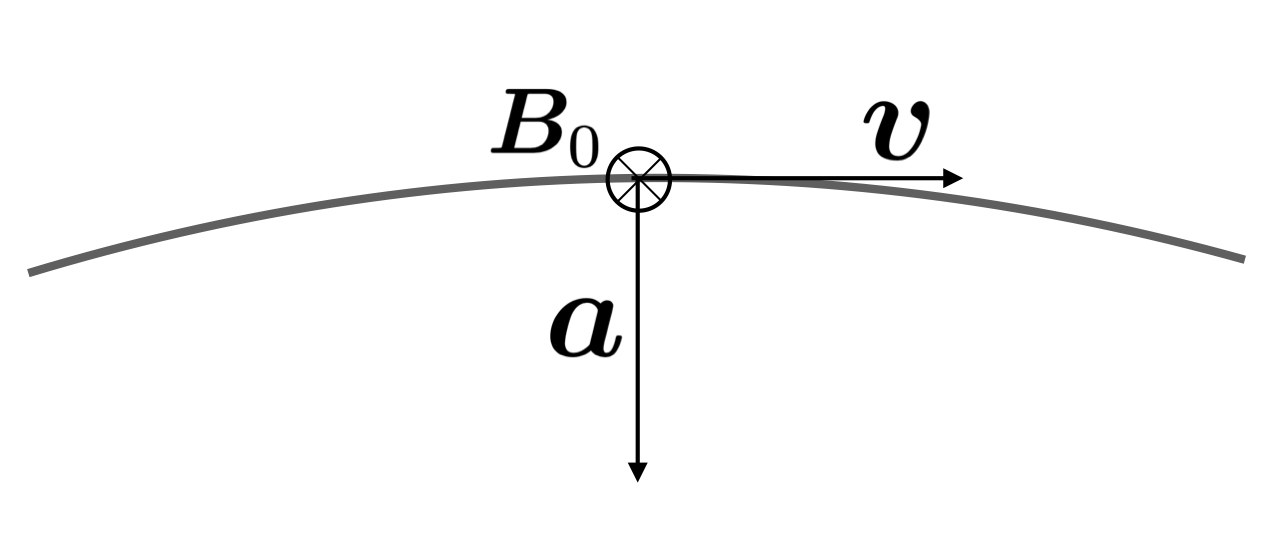
\includegraphics[scale=0.3]{Chapter-2/Figures/bending_mag_geo.png}
 \caption[Orientation of velocity, acceleration and applied magnetic field vectors for bending-magnet synchrotron radiation.]{Orientation of velocity, acceleration and applied magnetic field vectors ($\mathbold{v}$, $\mathbold{a}$ and $\mathbold{B}_0$, respectively) for bending-magnet synchrotron radiation. These vectors are each orthogonal to one another, with $\mathbold{B}_0$, which is produced by the bending magnet, pointing into the page. The gray curve represents an approximately-circular electron trajectory with a radius of curvature, $R$, such that $\mathbold{v}$ points tangentially and $\mathbold{a}$ points radially inward.}\label{fig:bending_magnet}. 
 \end{figure}
In principle, an electron in its rest frame radiates as a result of this centripetal acceleration according to the $\sin^2 \left( \vartheta \right)$ torus shape for \emph{Larmor radiation} shown in \cref{fig:torus_radition}. 
In the laboratory frame on the other hand, this radiation pattern is highly beamed along the direction of $\mathbold{v}$ (\emph{i.e.}, $\vartheta \approx 0$), where the opening angle scales with $\sqrt{1- \left( v / c_0 \right)^2}$, the inverse of the \emph{Lorentz factor} \cite{Attwood17}. 
Because $v \equiv \abs{\mathbold{v}}$ is constant in time for purely centripetal motion, the relativistic acceleration vector in \cref{eq:Lorentz_force_3} can be approximated as
\begin{subequations}
\begin{equation}\label{eq:Lorentz_accel_approx}
 \mathbold{a} = \frac{\mathbold{F}}{m_e} = \dv{t} \left( \frac{\mathbold{v}}{\sqrt{1-\frac{v^2}{c_0^2}}} \right) \approx \frac{1}{\sqrt{1-\frac{v^2}{c_0^2}}} \dv{\mathbold{v}}{t} .
 \end{equation}
The magnitude of the Lorentz force, $\abs{\mathbold{F}} = m_e \abs{\mathbold{a}}$, then can be written as 
\begin{equation}\label{eq:Lorentz_force_3_mag_approx}
 \frac{m_e}{\sqrt{1-\frac{v^2}{c_0^2}}} \underbrace{\abs{\dv{\mathbold{v}}{t}}}_{v^2/R_e} = \underbrace{\frac{m_e c_0^2}{\sqrt{1-\frac{v^2}{c_0^2}}}}_{\mathcal{E}_e^{\text{ALS}} \text{ by \cref{eq:ALS_energy}}} \underbrace{\frac{v^2}{c_0^2}}_{\approx 1}  R_e^{-1} = q_e v \abs{\mathbold{B}_0},
 \end{equation}
where $R_e$ is the radius of curvature associated with the electron trajectory, which is given by approximately by 
\begin{equation}
 R_e \approx \frac{\mathcal{E}_e^{\text{ALS}}}{q_e c_0 \abs{\mathbold{B}_0}} \approx \SI{5}{\metre}
 \end{equation}
with $v \approx c_0$ and $\abs{\mathbold{B}_0} \approx \SI{1.27}{\tesla}$ at the ALS \cite{Attwood17}. 
\end{subequations}
In addition to this beaming effect, bending-magnet radiation can be shown to have a broad spectrum due to the pulsed nature of electrons traveling in the storage ring.\footnote{Stated differently, \emph{Heisenberg's uncertainty principle} for energy and time states that a short, pulsed time interval leads to an appreciable spread of possible photon energies \cite[\emph{cf.\@} \cref{sec:gen_first_order}]{Attwood17}.} 
From derivations found in textbooks \cite{Attwood17,Jackson75}, the central wavelength in terms of radiated power across the emitted spectrum is given by 
\begin{equation}
 \lambda_c = \frac{4 \pi m_e}{3 q_e \abs{\mathbold{B}_0}} \approx \SI{0.407}{\nm} \quad \text{with } \abs{\mathbold{B}_0} \approx \SI{1.27}{\tesla}
 \end{equation}
for an ALS bending magnet, which corresponds to a \emph{tender x-ray} [\emph{cf.\@} \cref{sec:histroical}] with a photon energy of $\mathcal{E}_{\gamma} \approx \SI{3}{\kilo\electronvolt}$. 

Bending-magnet radiation that enters the grating monochromator system at beamline 6.3.2 is spectrally purified to produce a nearly monochromatic beam centered at a specified wavelength $\SI{40}{\nm} \gtrapprox \lambda \gtrapprox \SI{1}{\nm}$. 
Briefly, this system consists of a set of optics that focuses the synchrotron radiation before it is incident on an appropriately-ruled reflection grating that directs radiation at the blazed diffracted angle, $\beta = 2 \delta - \alpha$ [\emph{cf.\@} \cref{sec:grating_tech_intro}], through an exit slit, which is then refocused into a collimated beam \cite{Underwood96}. 
Radiation that passes through this system, however, must be spectrally filtered further with the use of of material slabs that have various spectral windows for transmission. 
Prominent absorption edges at EUV and soft x-ray wavelengths caused by these low-to-mid $\mathcal{Z}$ materials are also used for wavelength calibration procedures at the beamline. 
Moreover, the implementation of a triple-mirror order sorter is required to ensure spectral purity for radiation with $\lambda \gtrapprox \SI{2.8}{\nm}$ \cite{Gullikson01}. 
This beam of radiation ultimately is highly polarized along the vertical $y'$-direction labeled in \cref{fig:beamline_photoA}, which manifests as \emph{s-polarization} for an intercepting mirror flat\footnote{This refers to the electric field of the incident electromagnetic wave being perpendicular to plane of incidence and parallel to the surface. However, reflectivity is virtually polarization insensitive for grazing-incidence soft x-rays [\emph{cf.\@} \cref{sec:reflectivity_polarization}].} \cite{Muhlestein19}. 

As with any realistic source of radiation, the beam produced by the grating monochromator is associated with a finite coherence length, $\ell_{\text{coh}}$, that depends on $\lambda$ and a corresponding bandwidth, $\Delta \lambda$ [\emph{cf.\@} \cref{sec:coherent_states,fig:coherence_length}]. 
The grating monochromator at beamline 6.3.2 is reported to exhibit a relative spectral bandwidth of $\lambda / \Delta \lambda \lessapprox \num{7000}$ \cite{ALS_632,Underwood96,Gullikson01}, resulting in $\ell_{\text{coh}}$ on the order of \SI{10}{\um}. 
While the beam is mildly diverging with a cross-sectional diameter of $\lessapprox \SI{0.5}{\mm}$ at the optic mount, this level of coherence is sufficient for producing clearly-defined diffracted orders of wavelength $\lambda$, with locations given by \cref{eq:off-plane_orders} for a geometry parameterized by the incidence angles $\alpha$ and $\gamma$. 
\begin{figure}
 \centering
 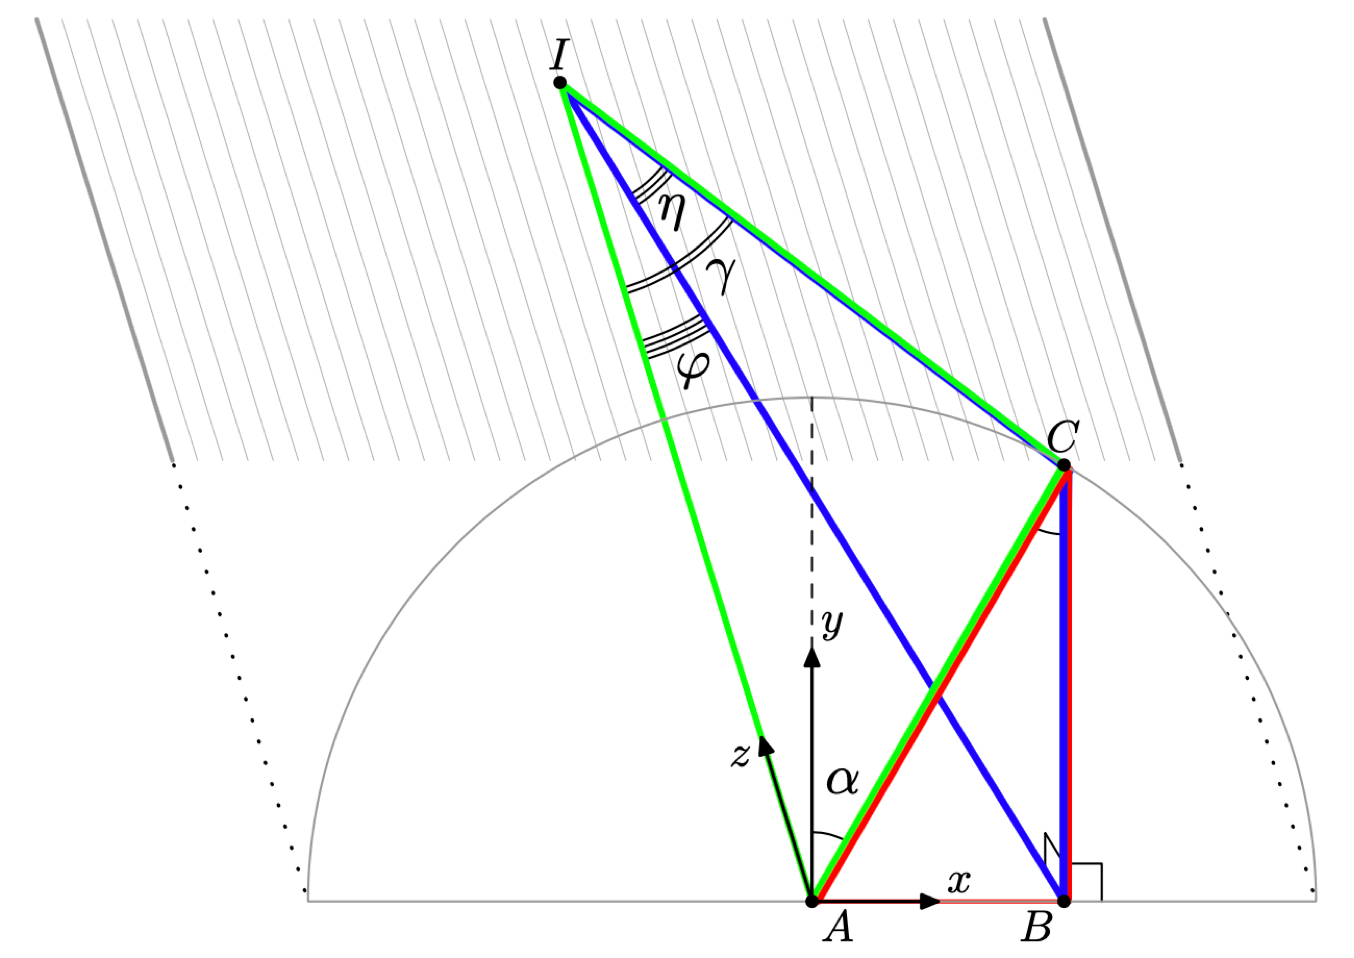
\includegraphics[scale=0.5]{Chapter-2/Figures/grating_angles.pdf}
 \caption[Angles relevant for beamline diffraction-efficiency testing]{Angles relevant for beamline diffraction-efficiency testing. The grating incidence angles $\alpha \equiv \angle ACB$ and $\gamma \equiv \angle AIC$ introduced in \cref{fig:conical_reflection_edit} are controlled through rotations about principal axes, which are parametrized by the angles $\eta \equiv \angle CIB$ and $\varphi \equiv \angle AIB$ given by \cref{eq:graze_angle,eq:yaw_angle} \cite{McCoy20}.}\label{fig:grating_angles} 
 \end{figure} 
Using the grating coordinate system defined in \cref{fig:grating_angles}, the central wave mode of the monochromatic beam with wave number $k_0 \equiv 2 \pi / \lambda$ has a wave vector written as 
\begin{subequations}
\begin{equation}\label{eq:beam_vec_grat}
 \mathbold{k} = k_x \mathbold{\hat{x}} + k_y \mathbold{\hat{y}} + k_z \mathbold{\hat{z}} = - k_0 \left[ \sin \left( \alpha \right) \sin \left( \gamma \right) \mathbold{\hat{x}} + \cos \left( \alpha \right) \sin \left( \gamma \right) \mathbold{\hat{y}} - \cos \left( \gamma \right) \mathbold{\hat{z}} \right] ,
 \end{equation}
whereas in the frame of the test chamber, this vector is taken to be oriented along the horizontal $z'$-direction labeled in \cref{fig:beamline_photoA} with 
\begin{equation}\label{eq:beam_vec_lab}
 \mathbold{k} = k_0 \mathbold{\hat{z}'} .
 \end{equation}
\end{subequations}
However, the implementation of the order sorter mentioned above shifts the beam direction so that $\mathbold{k}$ departs slightly from \cref{eq:beam_vec_grat,eq:beam_vec_lab}. 
Nonetheless, once a grating geometry has been established using the methodology outlined in \cref{sec:geo_constrain}, this beam can be used to measure $\mathscr{E}_n \! \left( \lambda \right)$ across a range of wavelengths [\emph{cf.\@} \cref{sec:measure_efficiency}]. 

\subsection{Constraining Grating Geometry}\label{sec:geo_constrain}
%%%%%%%%%%%%%%%%%%%%%%%%%%%%%%%%%%%%%%%%%--------------------------------------------------
Illustrated in \cref{fig:conical_reflection_edit}, angles $\alpha$ and $\gamma$ parameterize the direction of the incident radiation relative to the grating coordinate system defined in \cref{fig:grating_angles}, where $\mathbold{\hat{x}}$ is the grating-dispersion direction, $\mathbold{\hat{y}}$ is the cross-dispersion direction, and $\mathbold{\hat{z}}$ is the groove direction. 
At beamline 6.3.2, however, these angles are controlled indirectly through rotations about principal axes on the optic-mount stage \cite{Gullikson01,Miles18}. 
Two of these degrees of freedom are stage-controllable: the graze angle relative to the optic-mount surface, $\eta$, and another angle, $\varphi$, that describes the rotation of the grating about the axis normal to the optic-mount surface (\emph{i.e.}, grating yaw). 
As illustrated in \cref{fig:grating_angles}, the former angle is related to $\alpha$ and $\gamma$ through
\begin{equation}\label{eq:graze_angle}
 \sin \left( \eta \right) = \sin \left( \gamma \right) \cos \left( \alpha \right)
 \end{equation}
while, taking $\varphi = 90^{\circ}$ to correspond to an exact in-plane mount with $\sin \left( \gamma \right) = 1$, a relation for the latter can be written as 
\begin{equation}\label{eq:yaw_angle}
 \sin \left( \varphi \right) = \tan \left( \alpha \right) \tan \left( \eta \right) ,
 \end{equation}
or alternatively, $\cos \left( \varphi \right) = \cos \left( \gamma \right) / \cos \left( \eta \right)$ \cite{Miles18}.

The third degree of freedom (not shown in \cref{fig:grating_angles}) is an angle for grating roll, $\phi$, that nominally remains fixed at $\phi = 0$ so that the optic mount is leveled with $\eta = 0$. 
Although it is not stage-controllable, $\phi$ must be constrained experimentally along with $\eta$ and $\varphi$ to establish a near-Littrow configuration with $\alpha \approx \delta$ and $\gamma \approx \zeta < \zeta_c (\omega)$ at the beamline [\emph{cf.\@} \cref{eq:TER_condition_grat}]. 
This is done by first installing the grating on the optic mount, as shown in \cref{fig:beamline_photoB}, with $\eta \approx 0$ and $\phi \approx 0$ verified by the tilt of the optic mount using a spirit level. 
\begin{figure}
 \centering
 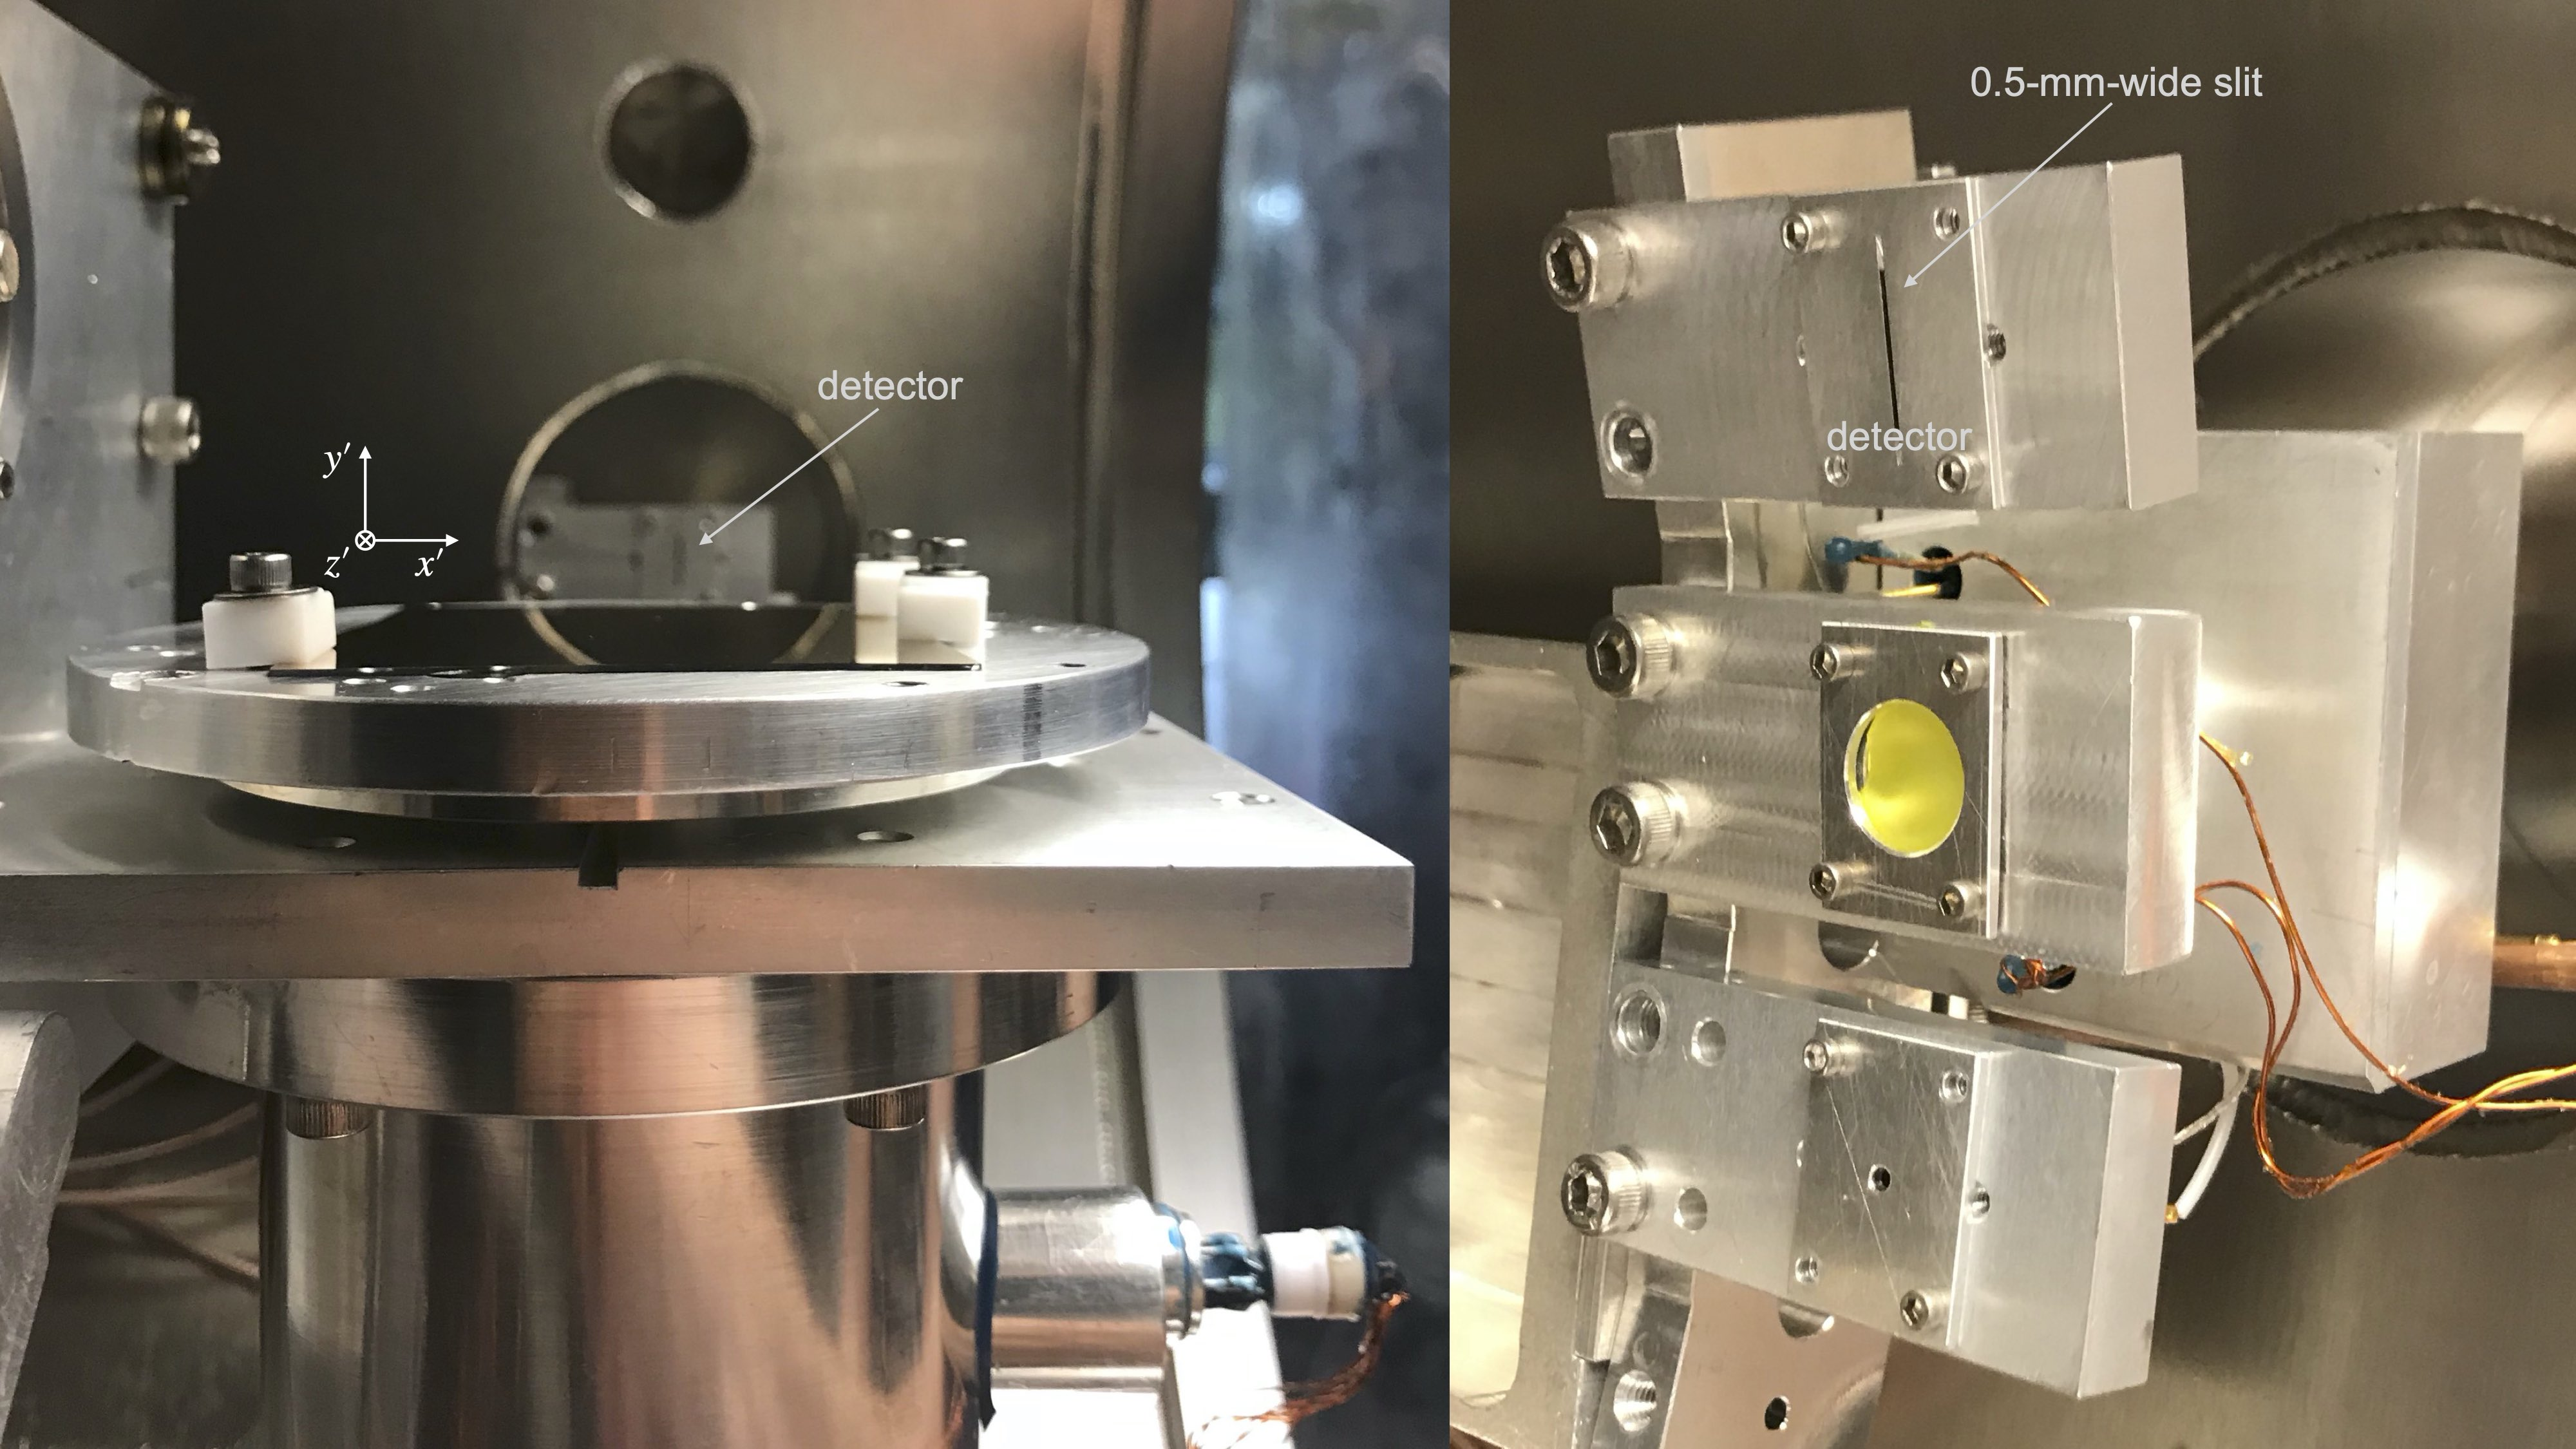
\includegraphics[scale=0.105]{Chapter-2/Figures/ALS_photoBC.jpg}
 \caption[View of the optic mount and masked photodiode detector at beamline 6.3.2 of the ALS]{Inside the test chamber shown in \cref{fig:beamline_photoA}, a \SI{0.5}{\mm}-wide, vertical slit is installed to mask the photodiode detector so as to allow the intensity of each propagating order, $\mathcal{I}_n \! \left( \lambda \right)$, to be measured in isolation. With the grating groove direction approximately aligned with the $z'$-axis for an extreme off-plane mount, the grating dispersion and cross-dispersion directions are approximately aligned with the linear $x'$-direction and the goniometric $y'$-direction motion of the detector staging, respectively.}\label{fig:beamline_photoB}
 \end{figure}
Meanwhile, the groove direction is approximately aligned with the beam direction with $\varphi \approx 0$ so that the $(x',y',z')$ chamber coordinate system [\emph{cf.\@} \cref{fig:beamline_photoA,fig:beamline_photoB}] is approximately coincident with the $(x,y,z)$ grating coordinate system [\emph{cf.\@} \cref{fig:grating_angles}]. 
The grating is then carefully adjusted to occult the beam so as to position the point of interception close to the hub of stage-rotation axes. 

With the leveled grating intercepting the beam, the optic mount can be rotated about the $x'$-axis at the point of incidence to ensure that the angle between the direct beam and the $0^{\text{th}}$-order beam is roughly $2 \eta$, where $\eta$ is the targeted graze angle [\emph{cf.\@} \cref{eq:graze_angle}]. 
The grating-dispersion direction, $\mathbold{\hat{x}}$, then is approximately parallel with the linear stage movement of the detector along the $x'$-direction so that the $x$-position of each propagating order [\emph{cf.\@} \cref{eq:linear_dispersion}] can be measured in a configuration with $\varphi \approx 0$ and $\phi \approx 0$ as
\begin{equation}\label{eq:disp_approx}
 x_n \approx x_0 + \frac{n \lambda L}{d} ,
 \end{equation}
where $x_0$ is the $x$-position of $0^{\text{th}}$ order. 
The ability to separate each component of $\mathcal{I}_n \! \left( \lambda \right)$, however, depends on the collecting-area dimensions of the detector used for data collection. 
That is, with $\lambda L / d$ typically on the order of \si{\mm} while the diffracted-arc radius [\emph{cf.\@} \cref{eq:blaze_wavelength}] is $r = L \sin \left( \gamma \right) \lessapprox \SI{8}{\mm}$ for $\gamma \lessapprox 2^{\circ}$, %eq:arc_radius
a detector with a narrow collecting area is required to allow each order to be measured in isolation. 
Moreover, if the detector length, $\ell_{\text{det}}$, is larger than $r$, $\mathcal{I}_n \! \left( \lambda \right)$ for each propagating order can be measured using purely horizontal detector motion with an appropriate choice for $\Theta$. 
Although this condition $\ell_{\text{det}} > r$ is not satisfied in both \cref{ch:master_fab,ch:grating_replication} due the use of detectors with different dimensions, a \SI{0.5}{\mm}-wide, vertical slit was in each case installed for the purposes of order separation [\emph{cf.\@} \cref{fig:beamline_photoB}]. %; an example of this is shown in \cref{fig:beamline_photoB}. 

For a grating geometry with zero yaw (\emph{i.e.}, $\varphi \approx 0$) and $\eta$ of a few degrees, \cref{eq:yaw_angle} requires that $\alpha \approx 0$ while the arc radius is given by $r \approx L \sin \left( \eta \right)$ [\emph{cf.\@} \cref{eq:arc_radius,eq:graze_angle}]. 
Increasing grating yaw by azimuthal stage rotation for $\varphi$ while $\eta$ remains fixed causes $\alpha$ to increase by \cref{eq:yaw_angle} and $r$ to increase as 
\begin{equation}
 r = L \sqrt{\sin^2 \left( \eta \right) + \sin^2 \left( \varphi \right) \cos^2 \left( \eta \right)} = L \sqrt{1 - \cos^2 \left( \varphi \right) \cos^2 \left( \eta \right)} .
 \end{equation}
A grating geometry with $\alpha \approx \delta$ hence can be established by setting $\eta$ and $\varphi$ appropriately according to \cref{eq:graze_angle,eq:yaw_angle} with $\phi \approx 0$. 
In principle, $L$ changes as the the detector moves along the $x'$-direction with focal corrections on the order of tens of \si{\um} within \si{mm} of detector travel, but for the analysis considered in this dissertation, these corrections are ignored so that $L$ is fixed for all detector positions considered. 
Order locations given by the generalized grating equation [\emph{cf.\@} \cref{eq:off-plane_orders,eq:off-plane_orders_ch2}] then can be mapped using $(x',y')$ positions associated with the detector staging that are taken to coincide directly with the $(x,y)$ coordinates for grating dispersion such that aberrations arising from the misalignment between these two planes are neglected. 
While the $x$-positions of propagating orders can be determined by sampling the diffracted arc along the $x'$-direction, their $y$-positions require knowledge of system throw, $L \approx \SI{235}{\mm}$ [\emph{cf.\@} \cref{fig:conical_reflection_edit}], to map the goniometric angle associated with the stage motion, $\Theta$, to a $y'$-coordinate using $y' = L \sin \left( \Theta \right)$ [\emph{cf.\@} \cref{fig:beamline_photoA}]. 

A measured value for $L$ can be measured experimentally by comparing the known detector length, $\ell_{\text{det}}$, 
\begin{figure}
 \centering
 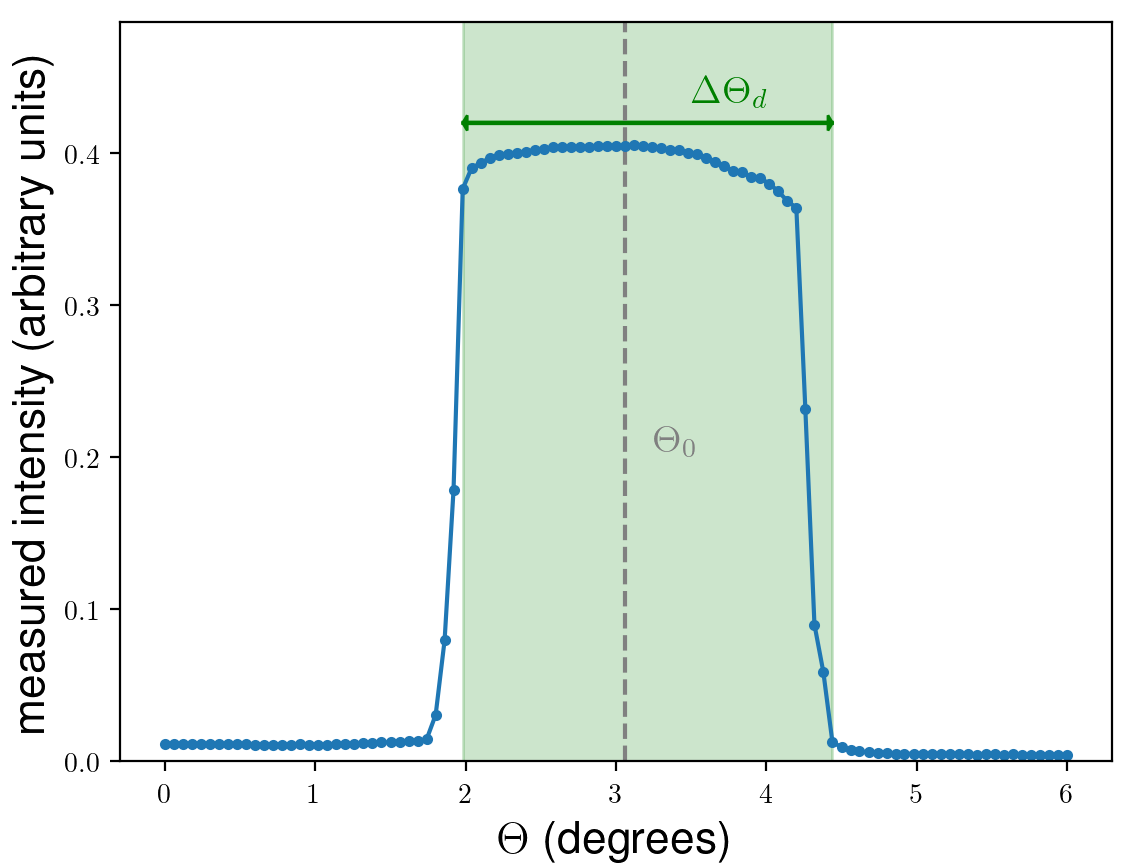
\includegraphics[scale=0.8]{Chapter-2/Figures/ALS_ydata_cent_range.png}
 \caption[Example of measured intensity data for a $0^{\text{th}}$-order diffracted beam as a function of goniometric angle]{Example of measured intensity data for a $0^{\text{th}}$-order diffracted beam as a function of goniometric angle, $\Theta$, in steps of $\sim$0.06$^{\circ}$. The green shaded region highlights the measured angular size of the detector, $\Delta \Theta_d$, which corresponds to one full translation of the beam in the goniometric direction, along the long direction of the \SI{0.5}{\mm}-wide slit. Additionally, the goniometric centroid angle associated with the measured beam, $\Theta_0$, can be determined through a weighted mean calculation of the data. This process is repeated for each propagating order to derive $\Theta_n$ for the $n^{\text{th}}$ order and ultimately, the corresponding $y$-component, $y_n = L \sin \left( \Theta_n \right)$.}\label{fig:ALS_cent_throw}
 \end{figure}
to the angular size of the detector as measured by a goniometric scan of the $0^{\text{th}}$-order beam, $\Delta \Theta_d$:
\begin{equation}
 \sin \left( \Delta \Theta_d \right) = \frac{\ell_{\text{det}}}{L} \implies L \approx \frac{\ell_{\text{det}}}{\Delta \Theta_d}
 \end{equation}
An example of this is shown in \cref{fig:ALS_cent_throw}, which depicts measured intensity data as a function of $\Theta$, in steps of $\sim$0.06$^{\circ}$. 
Using these data, a measurement for $\Delta \Theta_d$ can be extracted by identifying start and end points for $\Theta$ that correspond to one beam translation across the detector. 
This $\Theta$ range includes the quasi-flat region of the curve, where the full length of the beam falls on the detector, as well as one of its wings, which represents the beam either entering or exiting the active detector area. % [\emph{cf.\@} \cref{fig:ALS_cent_throw}]. 

With a measured value for $L$, a $y$-coordinate for any given diffracted beam can be determined by performing a goniometric scan at an appropriate $x'$-position and then extracting a centroid angle, $\Theta_n$, so that $y_n = L \sin \left( \Theta_n \right)$. 
This is shown for the case of $n=0$ in \cref{fig:ALS_cent_throw}, where a weighted-mean treatment of data is used to extract $\Theta_0$. 
The $x$-positions of propagating orders, on the other hand, require horizontal scans of the diffracted arc at a fixed goniometric angle so that centroids can be extracted. 
 %with an example shown in \cref{fig:ALS_xdata}. 
\begin{figure}
 \centering
 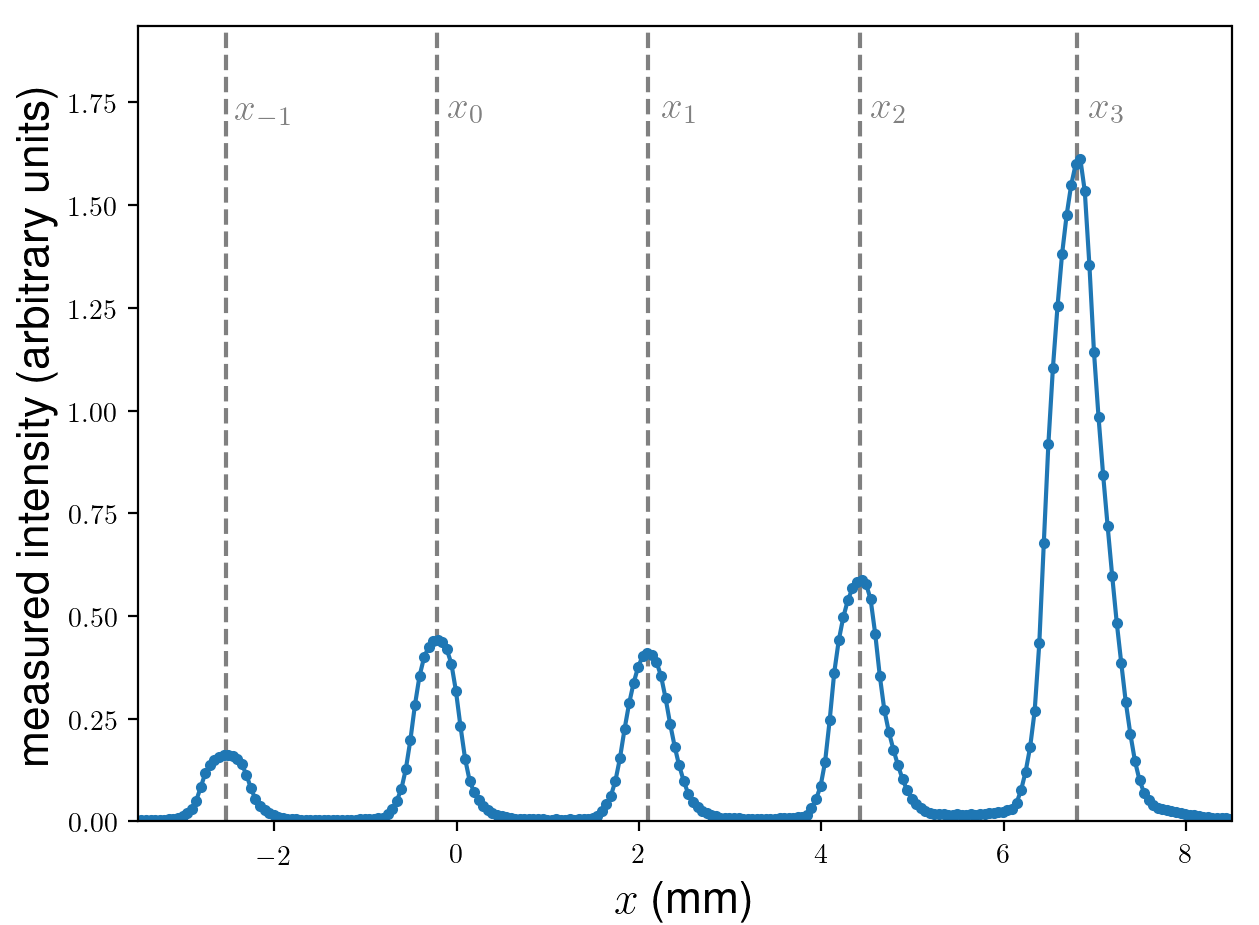
\includegraphics[scale=0.78]{Chapter-2/Figures/ALS_xdata.png}
 \caption[Example of measured intensity data for the diffracted arc as a function of horizontal detector position]{Example of measured intensity data for the diffracted arc as a function of horizontal detector position, $x'$, in steps of \SI{50}{\um}. The $x$-component of each propagating order, $x_n$, is determined using the weighted-mean centroid of each local maximum spaced approximately by $n \lambda L /d$.}\label{fig:ALS_xdata}
 \end{figure}
Example data that were gathered from a diffracted arc scanned horizontally in \SI{50}{\um} steps are shown in \cref{fig:ALS_xdata}, where a clear peak is seen for propagating orders with $n$ ranging from \numrange{-1}{3}. 
The weighted-mean centroid for each peak then yields an $x$-coordinate for the corresponding order [\emph{cf.\@} \cref{eq:disp_approx}] so that with $(x_n,y_n)$ measurements gathered for the diffracted arc, the data can be fit to a circle described by 
\begin{equation}\label{eq:arc_circle} 
 \left( x - x_{\text{cen}} \right)^2 + \left( y - y_{\text{cen}} \right)^2 = r^2,
 \end{equation}
where $(x_{\text{cen}},y_{\text{cen}})$ is the location of the arc center and $r = L \sin (\gamma)$ is its radius. 
\begin{figure}
 \centering
 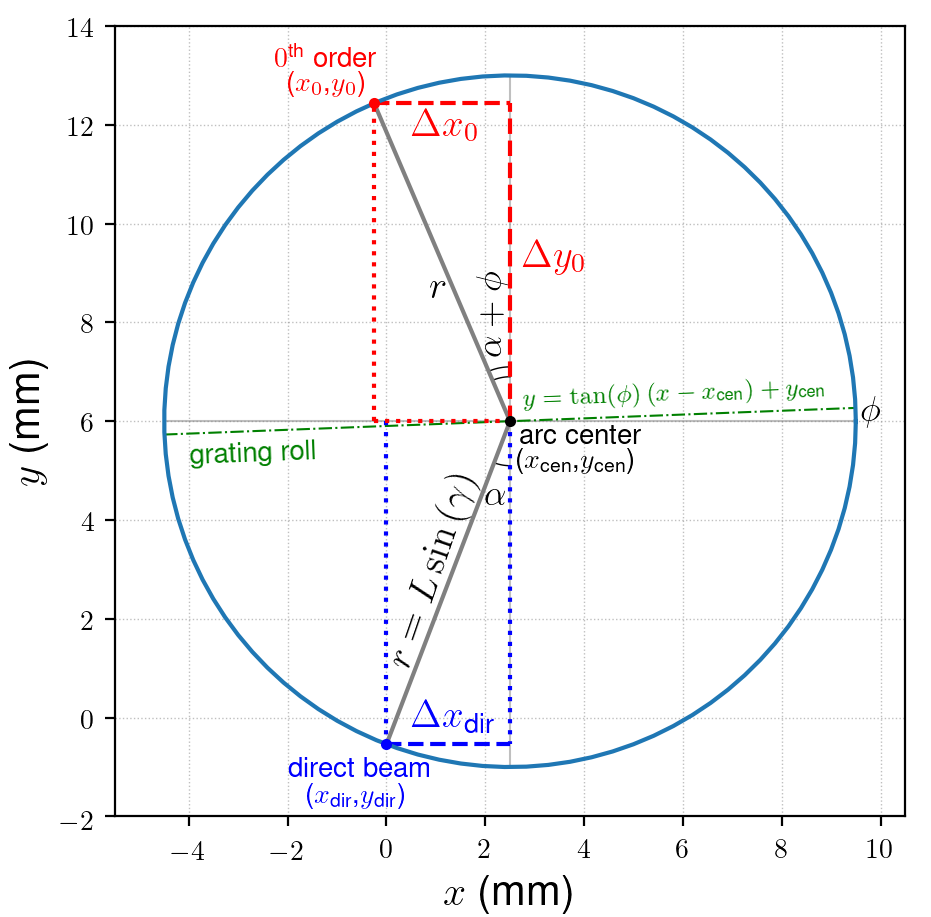
\includegraphics[scale=1.05]{Chapter-2/Figures/arc_example.png}
 \caption[Example of a diffracted arc fit to a circle]{Example of a diffracted arc fit to a circle by \cref{eq:arc_circle} with radius $r$ and arc center $(x_{\text{cen}},y_{\text{cen}})$ from gathered $(x_n,y_n)$ data. The cone opening half-angle, $\gamma$, is related to the system throw, $L$, through $r = L \sin \left( \gamma \right)$ while the azimuthal incidence angle, $\alpha$, follows from $\sin \left( \alpha \right) = \Delta x_{\text{dir}}/r$, where $\Delta x_{\text{dir}}$ is the $x$-distance between $x_{\text{cen}}$ and the direct beam. Grating roll, $\phi$, can be constrained using $\sin \left( \alpha + \phi \right) = \Delta x_0/r$, where $\Delta x_0$ is the $x$-distance between $x_{\text{cen}}$ and $0^{\text{th}}$ order. By \cref{eq:measure_graze}, the substrate graze angle, $\eta$, can be determined using the $y$-distance between $y_{\text{cen}}$ and $0^{\text{th}}$ order, $\Delta y_0$, while the angle for grating yaw, $\varphi$, follows from \cref{eq:measure_yaw}.}\label{fig:ALS_arc}
 \end{figure}
This is illustrated in \cref{fig:ALS_arc}, which depicts a circle of radius $r = \SI{7}{\mm}$ that represents an example diffracted arc with $\gamma \approx 1.7^{\circ}$. 

The positions of $0^{\text{th}}$ order, $(x_0,y_0)$, and the direct beam, $(x_{\text{dir}},y_{\text{dir}})$, are required along with $r$ and $(x_{\text{cen}},y_{\text{cen}})$ to constrain the angular degrees of freedom for the optic mount. 
By \cref{eq:arc_radius}, measured values for $L$ and $r$ yield the half-angle of the cone opening for the diffracted arc:
\begin{equation}\label{eq:measure_gamma}
 \gamma = \arcsin \left( \frac{r}{L} \right) \approx \frac{r}{L} , % + \frac{1}{6} \left( \frac{r}{L} \right)^3 ,
 \end{equation}
where the approximation holds for $r \ll L$. 
The azimuthal incidence angle, $\alpha$, then follows from \cref{eq:graze_angle} with a measured value for the graze angle relative to the grating substrate, $\eta$, which can be determined by comparing goniometric centroid angles for the direct beam and $0^{\text{th}}$ order with knowledge of grating roll \cite{Miles18}. 
Alternatively, this angle can be measured independently of $\gamma$ and $\eta$ using the $x$-distance between the direct beam and the arc center together with the arc radius [\emph{cf.\@} \cref{fig:ALS_arc}]:
\begin{equation}\label{eq:measure_alpha}
 \alpha = \arcsin \left( \frac{\Delta x_{\text{dir}}}{r} \right) ,
 \end{equation}
where $\Delta x_{\text{dir}} \equiv x_{\text{cen}} - x_{\text{dir}}$. 
While the angles $\alpha$ and $\gamma$ fully describe a conical grating geometry for the purposes of modeling diffraction efficiency in \cref{sec:integral_method}, the principle-axis angles defined in \cref{fig:grating_angles} should also be constrained to ensure consistency with \cref{eq:graze_angle,eq:yaw_angle}. 

By definition, a grating with zero roll is perfectly leveled with the $x'$-axis of the laboratory coordinate system so that $x_0 = x_{\text{dir}}$ and as a result, $\eta$ can be determined from $\sin \left( \eta \right) = \Delta y_0 / L$, where $\Delta y_0 \equiv y_0 - y_{\text{cen}}$ is the $y$-distance between $0^{\text{th}}$ order and the arc center. 
With a roll angle $\phi \lessapprox 1^{\circ}$, however, the diffracted arc is rotated slightly with $\Delta x_0 \equiv x_{\text{cen}} - x_0 > \Delta x_{\text{dir}}$. 
This angle can be determined using [\emph{cf.\@} \cref{fig:ALS_arc}] %As shown geometrically in \cref{fig:ALS_arc}, 
\begin{equation}\label{eq:measure_roll}
 \phi = \arcsin \left( \frac{\Delta x_0}{r} \right) - \alpha \approx \frac{\Delta x_0}{r} - \sin \left( \alpha \right) ,
 \end{equation}
where the approximation holds for $\abs{\Delta x_0 - \Delta x_{\text{dir}}} \ll r$. 
A nonzero roll also causes a measurement of $\Delta y_0$ to be underestimated by a factor of $\cos \left( \phi \right)$ such that 
a relation for $\eta$ is given by 
\begin{equation}\label{eq:measure_graze}
 \sin \left( \eta \right) = \frac{\Delta y_0 \sec \left( \phi \right)}{L} \implies \eta \approx \frac{\Delta y_0}{L} \left(1 + \frac{\phi^2}{2} \right)  .
 \end{equation}
Finally, $\varphi$ can be determined geometrically using the right triangle defined by $\Delta x_{\text{dir}}$ and the projection of the $0^{\text{th}}$-order ray into the plane of the grating, $L \cos \left( \eta \right)$, with $L$ as a hypotenuse:\footnote{This can be gleaned from \cref{fig:grating_angles}, where the line segment $\overline{IG}$ represents $L$ so that the line segment $\overline{IB}$ shown in solid blue is equivalent to $L \cos \left( \eta \right)$.}
\begin{equation}\label{eq:measure_yaw}
 \sin \left( \varphi \right) = \frac{\Delta x_{\text{dir}}}{L \cos \left( \eta \right)} \implies \varphi \approx \frac{\Delta x_{\text{dir}}}{L} \left(1 + \frac{\eta^2}{2} \right) ,
 \end{equation}
where the approximations in \cref{eq:measure_graze,eq:measure_yaw} hold for small angles. 

\subsection{Measuring Diffraction Efficiency}\label{sec:measure_efficiency}
%%%%%%%%%%%%%%%%%%%%%%%%%%%%%%%%%%%%%%%%%--------------------------------------------------
Once a desired grating geometry with $\alpha \approx \delta$ and $\gamma \approx \zeta < \zeta_c (\omega)$ has been established using the methodology described in \cref{sec:geo_constrain}, absolute diffraction efficiency, $\mathscr{E}_n$, can be experimentally determined according to \cref{eq:diffraction_efficiency} as function of wavelength, $\lambda$, or photon energy, $\mathcal{E}_{\gamma} \equiv h c_0 / \lambda$ with $h c_0 \approx \SI{1240}{\electronvolt\nm}$. 
For a given monochromatic-beam configuration, the intensity of each propagating order, $\mathcal{I}_n$, can be calculated by identifying the appropriate maxima from a horizontal detector scan [\emph{cf.\@} \cref{fig:ALS_xdata}] and then taking three measurements around the centroid after subtracting out the appropriate noise floors. 
Contributions to this noise include dark current from the photodiode detector, which can be measured using the detector readout in the absence of incident radiation, and diffuse scatter arising from surface roughness on the groove facets [\emph{cf.\@} \cref{sec:rough_surface}], which, in principle, can be estimated using the continuum level in between order maxima. 
The intensity of the direct beam, $\mathcal{I}_{\text{inc}}$, can be measured in a similar way while the optic mount is moved out of the beam path so that the only expected source of noise is dark current. 
These two processes for measuring $\mathcal{I}_n$ and $\mathcal{I}_{\text{inc}}$ can then be repeated as function of $\lambda$ (or $\mathcal{E}_{\gamma}$) using appropriate procedures for adjusting the monochromatic beam. 

Other useful quantities that characterize the performance of a reflection grating can be derived using measured data for $\mathscr{E}_n$ [\emph{cf.\@} \cref{eq:diffraction_efficiency}]. 
First, the \emph{total absolute diffraction efficiency} of a grating is defined as $\mathscr{E}_{\text{tot}} \equiv \sum_n \mathscr{E}_n$ for all propagating orders with $n \neq 0$. 
This quantity describes the fraction of radiation from a grating that is available for spectroscopy whereas the \emph{total response} of the grating, defined as $\mathscr{E}_{\text{tot}} + \mathscr{E}_0$, is a measure of all radiation that is \emph{specularly diffracted}\footnote{In analogy to a specularly-reflected beam from a mirror flat, this definition here is generalized to include propagating orders with diffracted angles described by the grating equation.} from the grating relative to the incident beam. 
In principle, $\mathscr{E}_{\text{tot}} + \mathscr{E}_0$, is equivalent to a measure of specular reflection from a mirror flat with a grazing-incidence angle equal to the groove facet incidence angle for a blazed grating, $\zeta$ [\emph{cf.\@} \cref{sec:refl_account}]. 
Moreover, the \emph{relative diffraction efficiency} of a reflection grating is defined as $\mathscr{E}_n / \mathcal{R}_F$, where $\mathcal{R}_F$ is the Fresnel reflectivity of an equivalent mirror flat at a grazing-incidence angle $\zeta$, which is virtually polarization insensitive at EUV and soft x-ray spectral wavelengths [\emph{cf.\@} \cref{sec:reflectivity_polarization}]. 
Related definitions are the \emph{total relative diffraction efficiency}, $\mathscr{E}_{\text{tot}} / \mathcal{R}_F$, and the \emph{total relative response}, $\left( \mathscr{E}_{\text{tot}} + \mathscr{E}_0 \right) / \mathcal{R}_F$. 
This latter quantity is a measure of all radiation lost to phenomena other than $\lambda$-dependent reflectivity, which includes, but is not limited to, the surface roughness effects described in \cref{sec:rough_surface}. 

\section{Modeling Diffraction Efficiency}\label{sec:integral_method}
%%%%%%%%%%%%%%%%%%%%%%%%%%%%%%%%%%%%%%%%%--------------------------------------------------
Basic physics of gratings are formulated according to a scalar theory of diffraction in \cref{sec:amplitude_phase}, where a reflection grating is treated as a surface of point-source emitters with periodically-varying phase (\emph{i.e.}, a \emph{phase grating}). 
Through performing a spatial Fourier transform of this periodic phase function, it is found that a sawtooth profile gives rise to an intensity pattern where diffraction efficiency is maximized near a certain \emph{blaze wavelength}, $\lambda_b$, for each propagating order [\emph{cf.\@} \cref{eq:blaze_wavelength,eq:blaze_wavelength_general}]. 
Although such a scalar treatment roughly describes the impact of groove shape on grating response, a vector theory of diffraction that takes into account rigorous boundary conditions at the surface of a grating is instead needed for predicting this behavior more accurately. 
With \cref{ch:master_fab,ch:grating_replication} utilizing the \textsc{PCGrate-SX} software package \cite{PCGrate_web} for this purpose, \cref{sec:grating_boundary} describes the general grating value problem while \cref{sec:grat_bound_consider} outlines how the integral method can be used to calculate relative diffraction efficiency under the simplifying assumption of a \emph{perfectly conducting} boundary. 
Finally, \cref{sec:refl_account} describes how the reflectivity phenomena outlined in \cref{sec:planar_interface} can be folded into these results to determine absolute diffraction efficiency. 

\subsection{The Grating Boundary Value Problem}\label{sec:grating_boundary}
%%%%%%%%%%%%%%%%%%%%%%%%%%%%%%%%%%%%%%%%%-------------------------------------------------
A time-harmonic boundary value problem that describes electromagnetic waves in the presence of a reflection grating can be formulated using framework similar to what is utilized in \cref{sec:planar_interface} for the ideal mirror flat and the pseudo-random rough surface. 
Using the Cartesian coordinate system from \cref{sec:geo_constrain} with $\mathbold{\hat{x}}$, $\mathbold{\hat{y}}$ and $\mathbold{\hat{z}}$ as unit vectors for the dispersion, cross-dispersion and groove directions, respectively,\footnote{Note that as in the case of the mirror flat described in \cref{sec:planar_interface}, the $y$-axis here is normal to the grating substrate. In this case, however, the $(x,z)$ coordinates are rotated relative to what is defined in \cref{fig:2Dmirror_angles,fig:in_plane_scatter,fig:off_plane_scatter} for the mirror flat, where $k_z = 0$ by convention.} the surface-relief profile of a grating can be understood as a special case of the framework for a rough surface presented in \cref{sec:rough_surface}, where the surface-profile function, $Y(x,z)$, is replaced by a specified \emph{groove function}, $g(x)$, which defines the cross-sectional shape of the grating groove profile. 
This function is assumed to be periodic over the groove spacing, $d$, so that $g(x) = g(x+d)$ and the function can be be expressed as a Fourier series with $K \equiv 2 \pi / d$ as the \emph{grating wave number} [\emph{cf.\@} \cref{eq:grating_number}]:
\begin{subequations}%http://mathworld.wolfram.com/FourierSeries.html
\begin{equation} \label{eq:groove_fourier_series}
 g(x) = \sum_{n=-\infty}^{\infty} g_n \mathrm{e}^{i n K x} \equiv \sum_{n=-\infty}^{\infty} g_n (x), 
 \end{equation} 
where the complex Fourier coefficients are given by
\begin{equation} \label{eq:groove_fourier_coeff}
 g_n = \frac{1}{d} \int_{0}^{d} g \left( x \right) \mathrm{e}^{- i n K x} \dd{x} \quad \text{for } n = 0, \pm 1, \pm 2, \pm 3 \dotsc 
 \end{equation} 
\end{subequations}
Meanwhile, the incident wave mode is taken to be the central wavelength, $\lambda$, of the monochromatic beam [\emph{cf.\@} \cref{sec:als_beam}] with a wave vector given by \cref{eq:beam_vec_grat}: 
\begin{subequations}
\begin{equation}\label{eq:beam_vec_grat_2}
 \mathbold{k} = k_x \mathbold{\hat{x}} + k_y \mathbold{\hat{y}} + k_z \mathbold{\hat{z}} = - k_0 \left[ \sin \left( \alpha \right) \sin \left( \gamma \right) \mathbold{\hat{x}} + \cos \left( \alpha \right) \sin \left( \gamma \right) \mathbold{\hat{y}} - \cos \left( \gamma \right) \mathbold{\hat{z}} \right] ,
 \end{equation}
where the angles $\alpha$ and $\gamma$ are defined geometrically in \cref{fig:grating_angles} and $k_0 \equiv 2 \pi / \lambda$.  
The accompanying wavefront, which is composed of an electric field, $\mathbold{E} \left( \mathbold{r} \right)$, and a magnetic field, $\mathbold{H} \left( \mathbold{r} \right)$, can be written in a form similar to \cref{eq:incident_fields}: 
\begin{equation} \label{eq:incident_fields_grat} 
 \mathbold{E} \left( x, y, z \right) = \mathbold{E}_0 \mathrm{e}^{i \left( k_x x + k_y y + k_z z \right)} \text{ and } \mathbold{H} \left( x, y, z \right) = \frac{1}{Z_0 k_0} \mathbold{k} \times \mathbold{E} \left( x, y, z \right) ,
 \end{equation}
\end{subequations}
where $Z_0$ is the impedance of free space and $\mathbold{E}_0 = E_{0,x} \mathbold{\hat{x}} + E_{0,y} \mathbold{\hat{y}} + E_{0,z} \mathbold{\hat{z}}$ has components  
\begin{subequations}
\begin{align}\label{eq:inc_E_comp}
 %\begin{split}
 E_{0,x} &= \mathcal{A}_0 \left[ \sin \left( \theta_p \right) \cos \left( \alpha \right) + \cos \left( \theta_p \right) \sin \left( \alpha \right) \cos \left( \gamma \right) \right] \\
 E_{0,y} &= \mathcal{A}_0 \left[ \cos \left( \theta_p \right) \cos \left( \alpha \right) \cos \left( \gamma \right) - \sin \left( \theta_p \right) \sin \left( \alpha \right) \right] \\
 E_{0,z} &= \mathcal{A}_0 \cos \left( \theta_p \right) \sin \left( \gamma \right) ,
 %\end{split}
 \end{align}
\end{subequations}
where $\mathcal{A}_0 \equiv \abs{\mathbold{E}_0}$ describes the amplitude of the electric field and the angle $\theta_p$ parameterizes the orientation of $\mathbold{E}_0 - E_{0,z} \mathbold{\hat{z}}$ relative to $\mathbold{k} - k_z \mathbold{\hat{z}}$ \cite[\emph{cf.\@} \cref{fig:polarization_angle}]{Petit80}. %projected onto the $(x,y)$ plane \cite{Petit80} [\emph{cf.\@} \cref{fig:polarization_angle}]. 

Similar to the treatment of specular reflectivity from a mirror flat [\emph{cf.\@} \cref{sec:reflectivity_polarization}], evaluating polarization sensitivity for a reflection grating can be handled by considering two special cases of \cref{eq:inc_E_comp} along with the corresponding amplitude vector for the magnetic field given by $\mathbold{H}_0 \equiv \left( Z_0 k_0 \right)^{-1} \mathbold{k} \times \mathbold{E}_0$. 
\begin{figure}
 \centering
 \includegraphics[scale=1.25]{Chapter-2/Figures/diffraction_arc26.mps}
 \caption[Definition of the polarization angle, $\theta_p$]{Definition of the polarization angle, $\theta_p$. The projection of the incident electric field amplitude, $\mathbold{E}_0$, onto the $(x,y)$ plane is represented by the unit vector $\hat{\mathbold{E}}_{xy}$, which is aligned with $\mathbold{E}_0 - E_{0,z} \mathbold{\hat{z}}$. This vector, along with the projection of $\mathbold{k}$ onto the $(x,y)$ plane given by $\mathbold{k}_{xy} \equiv \mathbold{k} - k_z \mathbold{\hat{z}} = - k_0 \sin \left( \gamma \right) \left[ \sin \left( \alpha \right) \mathbold{\hat{x}} + \cos \left( \alpha \right) \mathbold{\hat{y}} \right]$, define the angle $\theta_p$ with $\theta_p = 0$ and $\theta_p = \pi/2$ corresponding to transverse-electric (TE) and transverse-magnetic (TM) polarization, respectively.}\label{fig:polarization_angle}
 \end{figure} 
These are: $\theta_p  = 0$ such that the field amplitudes become
\begin{subequations}
\begin{align}
 \mathbold{E}_0 &= \mathcal{A}_0 \left[ \sin \left( \alpha \right) \cos \left( \gamma \right) \mathbold{\hat{x}} + \cos \left( \alpha \right) \cos \left( \gamma \right) \mathbold{\hat{y}} + \sin \left( \gamma \right) \mathbold{\hat{z}} \right] \\
 \mathbold{H}_0 &= \left( \frac{\mathcal{A}_0}{Z_0} \right) \left[ \cos \left( \alpha \right) \mathbold{\hat{x}} -  \sin \left( \alpha \right) \mathbold{\hat{y}} \right]
 \end{align}
\end{subequations}
and $\theta_p  = \pi/2$ such that
\begin{subequations}
\begin{align}
 \mathbold{E}_0 &= \mathcal{A}_0 \left[ \cos \left( \alpha \right) \mathbold{\hat{x}} - \sin \left( \alpha \right) \mathbold{\hat{y}} \right] \\
 \mathbold{H}_0 &= \left( \frac{\mathcal{A}_0}{Z_0} \right) \left[ \sin \left( \alpha \right) \cos \left( \gamma \right) \mathbold{\hat{x}} + \cos \left( \alpha \right) \cos \left( \gamma \right) \mathbold{\hat{y}} + \sin \left( \gamma \right) \mathbold{\hat{z}} \right] .
 \end{align}
\end{subequations}
The distinguishing feature between these two sets of equations is that $H_{0,z} = 0$ for $\theta_p  = 0$ while $E_{0,z} = 0$ for $\theta_p  = \pi/2$ and as a result, these two orthogonal polarizations are referred to as \emph{transverse-electric (TE) polarization} and \emph{transverse-magnetic (TM) polarization}, respectively \cite{Petit80,Loewen97}. 
Until \cref{sec:grat_bound_consider}, discussion centers on a generic case with $E_{0,z} \neq 0$ and $H_{0,z} \neq 0$. 

\subsubsection{Helmholtz Equation and Boundary Conditions}\label{sec:grating_Helmholtz}
%%%%%%%%%%%%%%%%%%%%%%%%%%%%%%%%%%%%%%%%%-------------------------------------------------
As generalizations of the reflection and refraction phenomena that occur from an incident wave striking an ideal mirror flat [\emph{cf.\@} \cref{sec:reflectivity_polarization}], \emph{reflected-diffracted} and \emph{refracted-diffracted} fields exist in the presence of a surface-relief grating along with the incident fields [\emph{cf.\@} \cref{eq:incident_fields_grat}]. % given by \cref{eq:incident_fields_grat}. 
While it will be shown that both sets of fields are split into propagating orders that depend on the order number $n$, they are first described generically using \cref{eq:3D_reflected_wave_vector} for the reflected-diffracted wave vector:
\begin{subequations}
\begin{equation}\label{eq:refl_diff_wave0}
 \mathbold{k''} = k_x'' \mathbold{\hat{x}} + k_y'' \mathbold{\hat{y}} + k_z'' \mathbold{\hat{z}} \quad \text{where} \quad k_0 = \sqrt{k_x''^2 + k_y''^2 + k_z''^2} , 
 \end{equation}
with \cref{eq:reflected_fields} for the reflected-diffracted fields:
\begin{equation}
\mathbold{E''} \left( x, y, z \right) = \mathbold{E}_0'' \mathrm{e}^{i \left( k_x'' x + k_y'' y + k_z'' z \right)} \text{ and } \mathbold{H''} \left( x, y, z \right) = \frac{1}{Z_0 k_0} \mathbold{k''} \times \mathbold{E''} \left( x, y, z \right) ,
 \end{equation} 
\end{subequations}
where $\mathbold{E}_0''$ describes polarization and amplitude in analogy to $\mathbold{E}_0$ for the incident wave. 
Similarly, \cref{eq:3D_refracted_wave_vector} is used for the complex refracted-diffracted wave vector that depends on the complex index of refraction of the grating material, $\tilde{\nu} (\omega)$: 
\begin{subequations}
\begin{equation}
 \mathbold{\tilde{k}'} = \tilde{k}_x' \mathbold{\hat{x}} + \tilde{k}_y' \mathbold{\hat{y}} + \tilde{k}_z' \mathbold{\hat{z}} \quad \text{where} \quad \tilde{\nu} (\omega) k_0 = \sqrt{\tilde{k}_x'^2 + \tilde{k}_y'^2 + \tilde{k}_z'^2} ,
 \end{equation}
with \cref{eq:refracted_fields} for the refracted-diffracted fields that decay as they propagate according to the imaginary parts of $\tilde{k}_x'$, $\tilde{k}_y'$ and $\tilde{k}_z'$:
\begin{equation}
 \mathbold{E'} \left( x, y, z \right) = \mathbold{E}_0' \mathrm{e}^{i \left( \tilde{k_x}' x + \tilde{k_y}' y + \tilde{k_z}' z \right)} \text{ and } \mathbold{H'} \left( x, y, z \right) = \frac{1}{Z_0 k_0} \mathbold{\tilde{k}'} \times \mathbold{E'} \left( x, y, z \right) ,
 \end{equation}
\end{subequations}
where $\mathbold{E}_0'$ describes polarization and the initial amplitude. 
Together, these fields must be solutions of the Helmholtz equation in vacuum [\emph{cf.\@} \cref{eq:Helmholtz_above_mirror}]: 
\begin{subequations}
\begin{equation}\label{eq:Helmholtz_above_mirror_ch2} 
 \left( \laplacian + k_0^2 \right) \left\{
 \begin{array}{lr}
 \mathbold{E} \left( x, y, z \right) + \mathbold{E''} \left( x, y, z \right) \\
 \mathbold{H} \left( x, y, z \right) + \mathbold{H''} \left( x, y, z \right) 
 \end{array}
 \right\} = \mathbf{0} \quad \text{for } y > g(x) ,
 \end{equation}
and inside the material of the grating [\emph{cf.\@} \cref{eq:Helmholtz_below_mirror}]:
\begin{equation}\label{eq:Helmholtz_below_mirror_ch2} 
 \left( \laplacian + \tilde{k}'^2 \right) \left\{
 \begin{array}{lr}
 \mathbold{E'} \left( x, y, z \right) \\
 \mathbold{H'} \left( x, y, z \right) 
 \end{array}
 \right\} = \mathbf{0} \quad \text{for } y < g(x) 
 \end{equation}
\end{subequations}
with $\tilde{k}' \equiv \tilde{\nu} (\omega) k_0$ and $\mathbf{0}$ as the null vector. 
\begin{figure}
 \centering
 \includegraphics[scale=1.25]{Chapter-2/Figures/diffraction_arc23.mps} 
 \caption[Surface-relief boundary between vacuum and a dispersive medium representing the functional material of a reflection grating]{Surface-relief boundary between vacuum and a dispersive medium representing the functional material of a reflection grating. With grooves aligned with the $z$-direction as in \cref{fig:grating_angles}, the cross-sectional profile, $\mathcal{P}$ (shown as a dashed line), of a grating with a groove spacing $d$ is described by the periodic function $g(x)$ confined to $0 \leq y \leq h$, where $h$ is the groove depth. The unit vector $\mathbold{\hat{n}}_{\mathcal{P}}(x)$ describes the direction normal to grating surface at a position $x$.}\label{fig:grating_boundary_def} 
 \end{figure}
They must also satisfy the appropriate boundary conditions at the surface of the grating profile, $\mathcal{P}$, described by $y = g(x)$, which can be written as special cases of \cref{eq:rough_boundary_1,eq:rough_boundary_2,eq:rough_boundary_3,eq:rough_boundary_4} for a rough surface with the pseudo-random function $Y(x,z)$ replaced by the periodic function $g(x)$:\footnote{These boundary conditions are valid in the absence of surface charge and surface current. This treatment is justified in the soft x-ray regime, where materials exhibit low electrical conductivity due to $\omega$ approaching their plasma frequency [\emph{cf.\@} \cref{sec:x-ray_index}]. For the scenario of a perfectly conducting grating described in \cref{sec:grat_bound_consider}, however, the refracted-diffracted fields are null and a term for surface current must be included.} 
\begin{subequations}
\begin{align}
 \mathbold{\hat{n}}_{\mathcal{P}}(x) \times \left[ \mathbold{E} \left( x, g(x), z \right) + \mathbold{E''} \left( x, g(x), z \right) \right] &= \mathbold{\hat{n}}_{\mathcal{P}}(x) \times \mathbold{E'} \left( x, g(x), z \right) \label{eq:grating_boundary_1} \\
 \mathbold{\hat{n}}_{\mathcal{P}}(x) \times \left[\mathbold{H} \left( x, g(x), z \right)  + \mathbold{H''} \left( x, g(x), z \right) \right] &= \mathbold{\hat{n}}_{\mathcal{P}}(x) \times \mathbold{H'} \left( x, g(x), z \right) \label{eq:grating_boundary_2} \\
 \mathbold{\hat{n}}_{\mathcal{P}}(x) \cdot \left[ \mathbold{E} \left( x, g(x), z \right) + \mathbold{E''} \left( x, g(x), z \right) \right] &= \tilde{\nu}^2 (\omega) \, \mathbold{\hat{n}}_{\mathcal{P}}(x) \cdot \mathbold{E'} \left( x, g(x), z \right) \label{eq:grating_boundary_3} \\
 \mathbold{\hat{n}}_{\mathcal{P}}(x) \cdot \left[ \mathbold{H} \left( x, g(x), z \right) + \mathbold{H''} \left( x, g(x), z \right) \right] &= \mathbold{\hat{n}}_{\mathcal{P}}(x) \cdot \mathbold{H'} \left( x, g(x), z \right)  \label{eq:grating_boundary_4} , 
 \end{align}
\end{subequations}
where $\mathbold{\hat{n}}_{\mathcal{P}}(x)$ 
is a unit vector normal to the grating surface at a position $x$ with $\mathbold{\hat{n}}_{\mathcal{P}}(x) \cdot \mathbold{\hat{z}} = 0$ [\emph{cf.\@} \cref{fig:grating_boundary_def}]. 

In analogy to the space-harmonic quality of an ideal mirror flat that leads to $k_{\parallel} = k_{\parallel}'' = \tilde{k_{\parallel}}'$ at a planar boundary [\emph{cf.\@} \cref{sec:reflectivity_polarization}], the fields on $\mathcal{P}$ have the property that a translation in $z$ introduces only a phase shift $\mathrm{e}^{i k_z z}$ to the incident fields: 
\begin{subequations}
\begin{equation}
 \left\{
 \begin{array}{lr}
 \mathbold{E} \left( x, y, z \right) \\
 \mathbold{H} \left( x, y, z \right)
 \end{array} 
 \right\} =  \left\{
 \begin{array}{lr}
 \mathbold{E} \left( x, y \right) \\
 \mathbold{H} \left( x, y \right)
 \end{array} 
 \right\} \mathrm{e}^{i k_z z} .
 \end{equation}
The boundary conditions given by \cref{eq:grating_boundary_1,eq:grating_boundary_2,eq:grating_boundary_3,eq:grating_boundary_4} then require $k_z = k_z'' = \tilde{k_z}'$ so that the reflected-diffracted and refracted-diffracted fields are given by 
\begin{equation}
 \left\{
 \begin{array}{lr}
 \mathbold{E}'' \left( x, y \right) \\
 \mathbold{H}'' \left( x, y \right)
 \end{array} 
 \right\} \mathrm{e}^{i k_z z} \quad \text{and} \quad   \left\{
 \begin{array}{lr}
 \mathbold{E}' \left( x, y \right) \\
 \mathbold{H}' \left( x, y \right)
 \end{array} 
 \right\} \mathrm{e}^{i k_z z} ,
 \end{equation}
\end{subequations}
respectively. 
These $\mathrm{e}^{i k_z z}$ terms the drop out of the Helmholtz equation so that, using the following shorthand notation: 
\begin{subequations}
\begin{align}
 \begin{split}
 \nabla_{xy}^2 \equiv \nabla^2 - \pdv[2]{z} &= \pdv[2]{x} + \pdv[2]{y} \quad \text{with} \\
 k_{xy}^2 \equiv k_0^2  - k_z^2 = k_x^2 + k_y^2 \quad &\text{and} \quad \tilde{k}_{xy}^2 \equiv \tilde{k}'^2 - \tilde{k_z}'^2 = \tilde{k_x}'^2 + \tilde{k_y}'^2 ,
 \end{split}
 \end{align} 
\end{subequations}
\cref{eq:Helmholtz_above_mirror_ch2} for vacuum reduces to 
\begin{subequations}
\begin{equation}\label{eq:Helmholtz_above_grating}
 \left( \nabla_{xy}^2 +  k_{xy}^2 \right) \left\{
 \begin{array}{lr}
 \mathbold{E} \left( x, y \right) + \mathbold{E''} \left( x, y \right) \\
 \mathbold{H} \left( x, y \right) + \mathbold{H''} \left( x, y \right) 
 \end{array}
 \right\} = \mathbf{0} \quad \text{for } y > g(x) 
 \end{equation}
and \cref{eq:Helmholtz_below_mirror_ch2} for the grating material reduces to 
\begin{equation}\label{eq:Helmholtz_below_grating}
 \left( \nabla_{xy}^2 + \tilde{k}_{xy}^2 \right) \left\{
 \begin{array}{lr}
 \mathbold{E'} \left( x, y \right) \\
 \mathbold{H'} \left( x, y \right) 
 \end{array}
 \right\} = \mathbf{0} \quad \text{for } y < g(x)  .
 \end{equation}
\end{subequations}

The framework just presented can be simplified for TE and TM polarization states by representing Faraday's law in time-harmonic form [\emph{cf.\@} \cref{eq:Maxwell_vac_TH_3}], $\curl \mathbold{E} \left( \mathbold{r} \right) = i \omega \mu_0 \mathbold{H} \left( \mathbold{r} \right)$, as 
\begin{subequations}
\begin{align}
 \pdv{E_z (x,y)}{y} - i k_z E_y (x,y) &= i \omega \mu_0 H_x (x,y) \label{eq:maxgrat1a} \\
 i k_z E_x (x,y) - \pdv{E_z (x,y)}{x} &= i \omega \mu_0 H_y (x,y) \label{eq:maxgrat1b} \\
 \pdv{E_y (x,y)}{x} - \pdv{E_x (x,y)}{y} &= i \omega \mu_0 H_z (x,y) \label{eq:maxgrat1bc} 
 \end{align}
\end{subequations}
and similarly, expressing the time-harmonic version of the Amp\`ere-Maxwell equation [\emph{cf.\@} \cref{eq:Maxwell_vac_TH_4}], $\curl \mathbold{H} \left( \mathbold{r} \right) = -i \omega \epsilon_0 \mathbold{E} \left( \mathbold{r} \right)$, as %without electric current,
\begin{subequations}
\begin{align}
 \pdv{H_z (x,y)}{y} - i k_z H_y (x,y) &= - i \omega \epsilon_0 E_x (x,y) \label{eq:maxgrat2a} \\
 i k_z H_x (x,y) - \pdv{H_z (x,y)}{x} &= - i \omega \epsilon_0 E_y (x,y) \label{eq:maxgrat2b} \\
 \pdv{H_y (x,y)}{x} - \pdv{H_x (x,y)}{y} &= - i \omega \epsilon_0 E_z (x,y) \label{eq:maxgrat2c} ,
 \end{align}
\end{subequations}
where, in both sets of equations, the factors of $k_z$ appear due to the the assumed $\mathrm{e}^{i k_z z}$ dependence along the groove direction. 
In the case of TE polarization with $H_z (x,y) = 0$, \cref{eq:maxgrat1a,eq:maxgrat1b,eq:maxgrat2a,eq:maxgrat2b} can be combined to give 
\begin{subequations}
\begin{align}
 \begin{split}\label{eq:TE_comps}
 \curl \left[ E_z (x,y) \mathbold{\hat{z}} \right] &= \frac{-i}{\omega \epsilon_0} k^2_{xy} \left[ H_x (x,y) \mathbold{\hat{x}} + H_y (x,y) \mathbold{\hat{y}} \right] \\
 &= \frac{-i}{k_z} k^2_{xy} \left[ E_x (x,y) \mathbold{\hat{x}} + E_y (x,y) \mathbold{\hat{y}} \right]
 \end{split}
 \end{align}
while for the case of TM polarization with $E_z (x,y) = 0$, these equations yield 
\begin{align}
 \begin{split}\label{eq:TM_comps}
 \curl \left[ H_z (x,y) \mathbold{\hat{z}} \right] &= \frac{-i}{\omega \mu_0} k^2_{xy} \left[ E_x (x,y) \mathbold{\hat{x}} + E_y (x,y) \mathbold{\hat{y}} \right] \\
 &= \frac{-i}{k_z} k^2_{xy} \left[ H_x (x,y) \mathbold{\hat{x}} + H_y (x,y) \mathbold{\hat{y}} \right] ,
 \end{split}
 \end{align}
\end{subequations}
where identical expressions hold for diffracted fields. 
Together, \cref{eq:TE_comps,eq:TM_comps} show that for the two orthogonal polarization states, the transverse component of the relevant field can be used to determine the remaining field components. 
With the incident wave being a solution to the Helmholtz equation by default, \cref{eq:Helmholtz_above_grating} reduces to a scalar equation for the relevant $z$-component of the fields for each polarization:
\begin{subequations}
\begin{equation}\label{eq:Helmholtz_above_grat_scal}
 \left( \nabla_{xy}^2 +  k_{xy}^2 \right) u'' (x,y) = 0 \quad \text{for } y > g(x) 
 \end{equation}
with 
\begin{equation}
 u'' (x,y) \equiv
   \begin{cases}
     E_z'' (x,y) & \text{for }\ \text{TE polarization} \\
     H_z'' (x,y) & \text{for }\ \text{TM polarization} 
   \end{cases} 
\end{equation}
\end{subequations}
and \cref{eq:Helmholtz_below_grating} for the grating material reduces to
\begin{subequations}
\begin{equation}\label{eq:Helmholtz_below_grat_scal}
 \left( \nabla_{xy}^2 + \tilde{k}_{xy}^2 \right) u' (x,y) = 0 \quad \text{for } y < g(x) 
 \end{equation}
with 
\begin{equation}
 u' (x,y) \equiv
   \begin{cases}
     E_z' (x,y) & \text{for }\ \text{TE polarization} \\
     H_z' (x,y) & \text{for }\ \text{TM polarization.} 
   \end{cases} 
\end{equation}
\end{subequations}
These two cases for the reflected-diffracted and refracted-diffracted fields are considered separately in \cref{sec:reflected_diffracted,sec:refracted_diffracted}. 

\subsubsection{Reflected-Diffracted Fields}\label{sec:reflected_diffracted}
%%%%%%%%%%%%%%%%%%%%%%%%%%%%%%%%%%%%%%%%%-------------------------------------------------
The condition $k_z = k_z''$ implies a $z$-direction law of reflection analogous to \cref{eq:reflection}, which ensures the cone opening half-angle to be equal to the angle $\gamma$ defined for the incident wave vector. 
This can be seen by writing the generic reflected-diffracted wave vector [\emph{cf.\@} \cref{eq:refl_diff_wave0,eq:3D_reflected_wave_vector}] as 
\begin{align}\label{eq:refl_diff_wave1}
 \begin{split}
 \mathbold{k''} &= k_x'' \mathbold{\hat{x}} + k_y'' \mathbold{\hat{y}} + k_z'' \mathbold{\hat{z}} \\
 &= k_0 \left[ \sin \left( \beta \right) \sin \left( \gamma'' \right) \mathbold{\hat{x}} + \cos \left( \beta \right) \sin \left( \gamma'' \right) \mathbold{\hat{y}} + \cos \left( \gamma'' \right) \mathbold{\hat{z}} \right] ,
 \end{split}
 \end{align}
where $\beta$ is the azimuthal diffracted angle [\emph{cf.\@} \cref{fig:conical_reflection_edit}] and $\gamma''$ is the cone opening half-angle: with $k_z = k_0 \cos \left( \gamma \right)$ by \cref{eq:beam_vec_grat}, $k_z = k_z''$ verifies $\gamma'' = \gamma$. 
The fields along the dispersion direction, on the other hand, experience a phase shift $\mathrm{e}^{i k_x x}$ due to incident wave and additionally, they are modulated by $\mathcal{P}$ defined by $g(x)$. 
Thus, with $\mathrm{e}^{i k_x x}$ accounted for, the relevant field component of the diffracted fields given by $u'' (x,y)$ can be expressed as a Fourier series similar to \cref{eq:groove_fourier_series} \cite{Petit80,antonakakis14}: 
\begin{subequations}
\begin{equation}\label{eq:refl_plane_spec_1}
  u'' \left[ x, g(x) \right] \mathrm{e}^{- i k_x x} = \sum_{n=-\infty}^{\infty} u_n'' \left[ g(x) \right] \mathrm{e}^{i n K x} ,
 \end{equation}
with $u_n'' (y)$ as an unknown function that describes the $n^{\text{th}}$ spatial harmonic of the diffracted field. 
Rewriting \cref{eq:refl_plane_spec_1} as
\begin{equation}\label{eq:refl_plane_spec_2}
 u'' \left[ x, g(x) \right] = \sum_{n=-\infty}^{\infty} u_n'' \left[ g(x) \right] \mathrm{e}^{i \left( k_x + n K \right) x} \equiv \sum_{n=-\infty}^{\infty} u_n'' \left[ g(x) \right] \mathrm{e}^{i k_{x,n}'' x} 
 \end{equation}
\end{subequations}
indicates that $k_x'' = k_x + n K \equiv k_{x,n}''$, which is recognized as the generalized grating equation [\emph{cf.\@} \cref{eq:off-plane_orders}].\footnote{This can be seen using $k_x'' = k_0 \sin \left( \beta \right) \sin \left( \gamma \right)$ from \cref{eq:refl_diff_wave1} and $k_x = - k_0 \sin \left( \alpha \right) \sin \left( \gamma \right)$ from \cref{eq:beam_vec_grat} with $k_0 \equiv 2 \pi / \lambda$ and $K \equiv 2 \pi / d$ such that from $k_x'' - k_x = nK$,
\begin{equation*}
 k_0 \sin \left( \gamma \right) \left[ \sin \left( \beta \right) + \sin \left( \alpha \right) \right] = nK \implies \sin \left( \alpha \right) + \sin \left( \beta \right) = \frac{n K}{k_0 \sin \left( \gamma \right)} = \frac{n \lambda}{d \sin \left( \gamma \right)} .
 \end{equation*}} 
The diffracted wave vector [\emph{cf.\@} \cref{eq:refl_diff_wave1}] then becomes 
\begin{align}
 \begin{split}\label{eq:refl_diff_wave2}
 \mathbold{k}_n'' &= k_{x,n}'' \mathbold{\hat{x}} + k_{y,n}'' \mathbold{\hat{y}} + k_z \mathbold{\hat{z}} \\
 \text{with} \quad k_{x,n}'' \equiv k_x &+ nK \quad \text{and} \quad k_{y,n}'' \equiv \sqrt{k_0^2 - \left( k_{x,n}''\right)^2 - k_z^2} , 
 \end{split}
 \end{align}
which shows that for all $n$ such that $k_0^2 > \left( k_x + nK \right)^2 + k_z^2$, there is a propagating order confined to the surface of a cone with opening angle $2 \gamma$ [\emph{cf.\@} \cref{sec:off-plane_geo}]. 

From the above considerations, the diffracted fields are expected to be of the form of a \emph{Rayleigh expansion}:
\begin{equation}\label{eq:refl_plane_spec_3}
 u'' (x,y) = \sum_{n=-\infty}^{\infty} u_n'' (y) \mathrm{e}^{i \left( k_x + n K \right) x} ,
 \end{equation}
which describes a \emph{spectrum of plane waves}, where $k_0$ remains constant but the direction of $\mathbold{k''}$ varies with $n$ so that the boundary conditions given by \cref{eq:grating_boundary_1,eq:grating_boundary_2,eq:grating_boundary_3,eq:grating_boundary_4} are satisfied \cite{Petit80,antonakakis14}. 
Inserting \cref{eq:refl_plane_spec_3} into \cref{eq:Helmholtz_above_grat_scal} and noting that the fields of the incident wave satisfy the Helmholtz equation by default gives 
\begin{align}\label{eq:Helmholtz_above_grating_expand}
 \begin{split}
 \left( \nabla_{xy}^2 +  k_{xy}^2 \right) \sum_{n=-\infty}^{\infty} u_n'' (y) \mathrm{e}^{i \left( k_x + n K \right) x}  &= 0 \\
 \implies \sum_{n=-\infty}^{\infty} \left[ \dv[2]{u_n'' (y)}{y} + \left( k_{y,n}'' \right)^2 u_n'' (y) \right] \mathrm{e}^{i n K x} &= 0 ,
 \end{split}
 \end{align}
where the phase factor $\mathrm{e}^{i k_x x}$ drops out of the second line. For $y > h \equiv \text{max} \! \left[g(x)\right]$ such that $\tilde{\nu} (\omega) = 1$ holds for all $x$, \cref{eq:Helmholtz_above_grating_expand} reduces to a collection of differential equations for each value of $n$ \cite{Petit80,antonakakis14}:\footnote{Fields in the grooved region with $0 \leq y \leq h$ are considered in \cref{sec:grat_bound_consider}.}
\begin{equation}\label{eq:Helmholtz_above_grating_order}
 \dv[2]{u_n'' (y)}{y} + \left( k_{y,n}'' \right)^2 u_n'' (y) = 0 .
 \end{equation}
A physically-realistic solution to \cref{eq:Helmholtz_above_grating_order} is one which diffracted waves propagate away from the grating surface, in vacuum:
\begin{subequations}
\begin{equation}\label{eq:Helmholtz_above_grat_order_sol}
  u_n'' (y) = \mathcal{U}_n'' \mathrm{e}^{i k_{y,n}'' y}
 \end{equation}
with
\begin{equation}\label{eq:generic_amp}
 \mathcal{U}_n'' \equiv
   \begin{cases}
     \mathcal{A}_{\text{TE},n}'' \sin \left( \gamma \right) & \text{for } \text{TE polarization} \\
     Z_0^{-1} \mathcal{A}_{\text{TM},n}'' \sin \left( \gamma \right) & \text{for } \text{TM polarization,} 
   \end{cases} 
\end{equation}
\end{subequations}
where $\mathcal{A}_{\text{TE},n}''$ and $\mathcal{A}_{\text{TM},n}''$ are the electric-field amplitudes of the $n^{\text{th}}$ order in each orthogonal polarization while $Z_0$ is the impedance of free space. 
The total diffracted field then can be written as a sum of diffracted orders:
\begin{equation}\label{eq:diff_field_exp}
u'' (x,y) = \sum_{n=-\infty}^{\infty} \mathcal{U}_n'' \mathrm{e}^{i \left( k_{x,n}'' x + k_{y,n}'' y \right)} ,
 \end{equation}
which results from combining \cref{eq:refl_plane_spec_3,eq:Helmholtz_above_grat_order_sol}. 

In analogy to the definition of specular reflectivity [\emph{cf.\@} \cref{eq:fresnel_refl_def}], the diffraction efficiency in each orthogonal polarization is defined as the outgoing flux of propagating orders through an imagined surface above the grating substrate relative to the incoming flux associated with the incident wave [\emph{cf.\@} \cref{eq:diffraction_efficiency}]. 
By defining a scalar function for the $z$-component of the incident field as
\begin{subequations}
\begin{equation}
 u (x,y) \equiv \left\{
 \begin{array}{lr}
  E_z (x,y) \\
  H_z (x,y)
 \end{array}
 \right\} \equiv \mathcal{U}_0 \mathrm{e}^{i \left( k_x x + k_y y \right)}  
\end{equation}
with 
\begin{equation}
 \mathcal{U}_0 \equiv
   \begin{cases}
     \mathcal{A}_0 \sin \left( \gamma \right) & \text{for } \text{TE polarization} \\
     Z_0^{-1} \mathcal{A}_0 \sin \left( \gamma \right) & \text{for } \text{TM polarization,} 
   \end{cases} 
\end{equation}
\end{subequations}
these quantities can be expressed as 
\begin{subequations}
\begin{align}
 \mathscr{E}_{\text{TE},n} &= \frac{k_{y,n}''}{k_y} \norm{\frac{\mathcal{A}_{\text{TE},n}''}{\mathcal{A}_0}}^2 = \frac{\cos \left( \beta \right)}{\cos \left( \alpha \right)} \norm{\tilde{r}_{\text{TE}}^{(n)}}^2\label{eq:TE_efficiency} \\ 
 \mathscr{E}_{\text{TM},n} &= \frac{k_{y,n}''}{k_y} \norm{\frac{\mathcal{A}_{\text{TM},n}''}{\mathcal{A}_0}}^2 = \frac{\cos \left( \beta \right)}{\cos \left( \alpha \right)} \norm{\tilde{r}_{\text{TM}}^{(n)}}^2 ,
 \end{align} 
where $\mathcal{A}_0$ is the amplitude of the incident electric field [\emph{cf.\@} \cref{eq:inc_E_comp,fig:polarization_angle}] while $\tilde{r}_{\text{TE}}^{(n)} \equiv \mathcal{A}_{\text{TE},n}'' / \mathcal{A}_0$ and $\tilde{r}_{\text{TM}}^{(n)} \equiv \mathcal{A}_{\text{TE},n}'' / \mathcal{A}_0$ are unitless amplitude coefficients that are generally complex. 
Diffraction efficiency for an arbitrary polarization state can then be written as 
\begin{equation}\label{eq:diffraction_efficiency_theo}
 \mathscr{E}_n = \mathscr{E}_{\text{TE},n} \cos^2 \left( \theta_p \right) + \mathscr{E}_{\text{TM},n} \sin^2 \left( \theta_p \right) ,
 \end{equation}
\end{subequations}
where $\theta_p$ is the polarization angle \cite[\emph{cf.\@} \cref{eq:inc_E_comp,fig:polarization_angle}]{Petit80}. 
Determining amplitude coefficients $\mathcal{A}_{\text{TE},n}''$ and $\mathcal{A}_{\text{TM},n}''$ follows from enforcing boundary conditions for a given polarization state [\emph{cf.\@} \cref{sec:grat_bound_consider}]. 

\subsubsection{Refracted-Diffracted Fields}\label{sec:refracted_diffracted}
%%%%%%%%%%%%%%%%%%%%%%%%%%%%%%%%%%%%%%%%%-------------------------------------------------
In analogy to Snell's law of refraction for a planar interface [\emph{cf.\@} \cref{eq:refraction}], the requirement $k_z = \tilde{k_z}'$ yields a relationship between $\gamma$ and the cone opening half-angle of refracted-diffracted radiation. 
The complex, refracted-diffracted wave vector can be written as
\begin{align}
 \begin{split}\label{eq:refr_diff_wave1}
 \mathbold{\tilde{k}'} &= \tilde{k}_x' \mathbold{\hat{x}} + \tilde{k}_y' \mathbold{\hat{y}} + \tilde{k}_z' \mathbold{\hat{z}} \\
 &=  \tilde{k}' \left[ \sin \left( \tilde{\beta}' \right) \sin \left( \tilde{\gamma}' \right) \mathbold{\hat{x}} - \cos \left( \tilde{\beta}' \right) \sin \left( \tilde{\gamma}' \right) \mathbold{\hat{y}} + \cos \left( \tilde{\gamma}' \right) \mathbold{\hat{z}} \right] ,
 \end{split}
 \end{align}
where $\tilde{\beta}'$ and $\tilde{\gamma}'$ are complex angles that, for propagating orders, have real components that represent the diffracted angle and cone opening half-angle, respectively, and imaginary components that are related to wave attenuation in the material, as described in \cref{sec:total_refl} for the case of a mirror flat.\footnote{The geometry for conical diffraction from a transmission grating is illustrated in \cref{fig:conical_transmission}. However, this figure neglects effects related to refraction and hence the diffracted angle and the cone opening half-angle are labeled as $\beta$ and $\gamma$, respectively.} 
From $k_z = k_0 \cos (\gamma)$ and $k_z = \tilde{k}' \cos \left( \tilde{\gamma}' \right)$, the relevant form of Snell's law along the $z$-direction is 
\begin{subequations}
\begin{equation}\label{eq:comp_snell_grat}
\cos \left( \gamma \right) = \tilde{\nu}(\omega) \cos \left( \tilde{\gamma}' \right) ,
 \end{equation}
which can be decomposed into two expressions as in \cref{eq:refractionA,eq:refractionB}:
\begin{align}
 \nu (\omega) \cos \left( \gamma'_{\Re} \right) \cosh \left( \gamma'_{\Im} \right) + \xi (\omega) \sin \left( \gamma'_{\Re} \right) \sinh \left( \gamma'_{\Im} \right) &= \cos \left( \zeta \right) \label{eq:refractionA_grat} \\
 \xi (\omega) \cos \left( \gamma'_{\Re} \right) \cosh \left( \gamma'_{\Im} \right) - \nu (\omega) \sin \left( \gamma'_{\Re} \right) \sinh \left( \gamma'_{\Im} \right) &=0 \label{eq:refractionB_grat} ,
 \end{align} 
\end{subequations} 
where $\tilde{\gamma}' \equiv \gamma'_{\Re} + i \gamma'_{\Im}$ and $\tilde{\nu} (\omega) \equiv \nu (\omega) + i \xi (\omega)$. 
These equations imply that if $\xi (\omega)$ can be neglected, $\gamma'_{\Im} = 0$ with \cref{eq:comp_snell_grat} reducing to a purely real equation similar to \cref{eq:Snell_real}:\footnote{As described in \cref{sec:total_refl}, the effect of $\xi (\omega) \neq 0$ causes the fields to penetrate slightly into the material with $\gamma'_{\Re}$ being a small angle given approximately by \cref{eq:zetaprime_real} with $\zeta \to \gamma$.}
\begin{equation}\label{eq:Snell_real_grat}
 \cos \left( \gamma \right) = \nu (\omega) \cos \left( \gamma'_{\Re} \right) .
 \end{equation}
TER in an extreme off-plane geometry is enabled for values of $\gamma$ that yield $\gamma'_{\Re} = 0$ by \cref{eq:Snell_real_grat}. 
However, the topography of the grating grooves must also be taken into account; for a blazed grating with an active facet angle $\delta$, the angle on the groove facet, $\zeta$, must be smaller than the critical angle for TER [\emph{cf.\@} \cref{eq:TER_condition_grat}]. 

In any case where radiation is considered to penetrate into the grating material, the refracted fields on $\mathcal{P}$ take on the periodicity of the grating as in \cref{sec:reflected_diffracted} for the reflected fields. 
This can be written analogously to \cref{eq:refl_plane_spec_1} as 
\begin{subequations}
\begin{equation}\label{eq:refr_plane_spec_1}
  u' \left[ x, g(x) \right] \mathrm{e}^{- i k_x x} = \sum_{n=-\infty}^{\infty} u_n' \left[ g(x) \right] \mathrm{e}^{i n K x} ,
 \end{equation}
$u' (x,y)$ is either $E_z' (x,y)$ or $H_z' (x,y)$ depending on polarization and $u_n' (y)$ is an unknown function that describes the $n^{\text{th}}$ spatial harmonic of the diffracted field. 
As in \cref{sec:reflected_diffracted}, \cref{eq:refr_plane_spec_1} indicates a spectrum of planes waves for $y <0$:
\begin{equation}\label{eq:refr_plane_spec_2} %for the case of reflected-diffracted fields
 u' (x,y) = \sum_{n=-\infty}^{\infty} u_n' (y) \mathrm{e}^{i \left( k_x + n K \right) x} \equiv \sum_{n=-\infty}^{\infty} u_n' (y) \mathrm{e}^{i \tilde{k}_{x,n}' x} ,
 \end{equation}
\end{subequations}
where the expression $\tilde{k}_x' = k_x + n K \equiv \tilde{k}_{x,n}'$ is recognized as the \emph{grating equation in a dispersive medium}:\footnote{This can be seen using $\tilde{k_x}' = \tilde{k}' \sin \left( \tilde{\beta}' \right) \sin \left( \tilde{\gamma}' \right)$ from \cref{eq:refr_diff_wave1} and $k_x = - k_0 \sin \left( \alpha \right) \sin \left( \gamma \right)$ from \cref{eq:beam_vec_grat} along with \cref{eq:comp_snell_grat} to eliminate $\tilde{\gamma}'$.}  
\begin{equation}\label{eq:grat_disp_med}
 \sin \left( \alpha \right) \sin \left( \gamma \right) + \sin \left( \tilde{\beta}' \right) \sqrt{\tilde{\nu}^2 \left( \omega \right) - \cos^2 \left( \gamma \right)} = \frac{n \lambda}{d} . 
 \end{equation}
The diffracted wave vector given by \cref{eq:refr_diff_wave1} then becomes 
\begin{align}
 \begin{split}
 \mathbold{\tilde{k}}_n' &= \tilde{k}_{x,n}' \mathbold{\hat{x}} + \tilde{k}_{y,n}' \mathbold{\hat{y}} + k_z \mathbold{\hat{z}} \\
 \text{with} \quad \tilde{k}_{x,n}'  \equiv k_x &+ nK \quad \text{and} \quad \tilde{k}_{y,n}'  \equiv \sqrt{\tilde{k}'^2 - \left( \tilde{k}_{x,n}'  \right)^2 - k_z^2},
 \end{split}
 \end{align} 
which describes a decaying, propagating order for all $n$ at which yield $\abs{\Re \left[ \tilde{\beta}' \right]} < 90^{\circ}$ according to \cref{eq:grat_disp_med}. 
Meanwhile, $\Im \left[ \tilde{\beta}' \right]$ is related to the attenuation of a diffracted ray that, in analogy to the case of a mirror flat [\emph{cf.\@} \cref{sec:total_refl}], causes electromagnetic waves to be highly distorted as they propagate and decay in nearly orthogonal directions. 
The \emph{penetration depth}, $\mathcal{D}_{\perp}$, defined by \cref{eq:penetration_depth} as the vertical distance into a material over which the intensity of radiation drops to $1/\mathrm{e}$ its initial value, informs thickness requirements for reflective overcoats on gratings. 
That is, with a thickness of \numrange{4}{5} $\mathcal{D}_{\perp}$, reflections at underlying material interfaces can be neglected and the layer can be considered virtually infinitely thick. 
For a high-$\mathcal{Z}$ material such as gold, this thickness requirement is $\sim \SI{15}{\nm}$ for grazing-incidence soft x-rays [\emph{cf.\@} \cref{fig:X-ray_atten}]. 

\subsection{The Integral Method for X-ray Reflection Gratings}\label{sec:grat_bound_consider}
%%%%%%%%%%%%%%%%%%%%%%%%%%%%%%%%%%%%%%%%%-------------------------------------------------
The grating boundary value problem presented in \cref{sec:grating_boundary} can be simplified with two assumptions that are justified in the following discussion:
\begin{enumerate}[noitemsep]
	\item The grating medium is considered to be \emph{perfectly conducting} such that the refracted fields are null with $\mathbold{E'} \left( x, y \right) = \mathbold{H'} \left( x, y \right) = \mathbf{0}$
	\item Diffraction efficiency is polarization insensitive for x-ray reflection gratings but with the assumption of perfect conductivity, gratings are modeled most accurately using TE polarization \cite{Marlowe16}
 \end{enumerate}
Although real materials are poorly conducting at soft x-ray frequencies for the reasons outlined in \cref{sec:SXR_med}, the electromagnetic fields involved in lossless TER behave similarly to those striking a medium with perfect conductivity, where the \emph{skin depth}\footnote{In a conducting medium with permittivity, permeability and conductivity given by $\epsilon$, $\mu$ and $\sigma$, respectively, solving Maxwell's equations using Ohm's Law given by $\mathbfcal{J} = \sigma \mathbold{E}$, with $\mathbfcal{J}$ as current density, yields $\tilde{k}^2 = k^2 + i \mu \sigma \omega$ as dispersion relation with $k \equiv \omega \sqrt{\epsilon \mu}$ and $\tilde{k}$ as a complex wave number. For very high conductivity or very low frequencies, the skin depth, which describes the distance over which the fields to $1/\mathrm{e}$ their initial amplitude, is given by 
\begin{equation*}
 \mathcal{D}_{\sigma} \approx \sqrt{\frac{2}{\omega \mu \sigma}} ,
 \end{equation*}
which approaches zero as $\sigma \to \infty$ \cite{Landau60}.\label{footnote:skin_depth}}
approaches zero \cite{Griffiths17,Jackson75}. 
This can be understood by considering that the refracted angle at an interface between vacuum and a dispersive medium with index of refraction $\tilde{\nu}(\omega) = \nu (\omega) + i \xi (\omega)$ is null for TER in the limit that $\xi (\omega) \to 0$ [\emph{cf.\@} \cref{sec:total_refl}]. 
Under such conditions, the fields do not penetrate into the dispersive medium so that the penetration depth, $\mathcal{D}_{\perp}$, approaches zero while Fresnel reflectivity, $\mathcal{R}_F$, is unity. 
While this assumption is not strictly justified for TER in the soft x-ray, where $\mathcal{D}_{\perp}$ is on the order of a few \si{\nm} and $\mathcal{R}_F<1$ [\emph{cf.\@} \cref{sec:planar_interface}], it has been demonstrated experimentally that x-ray reflection gratings used in the extreme off-plane mount exhibit polarization-insensitive diffraction efficiency that can be modeled with a fair degree of accuracy using the assumption of perfect conductivity \cite{Marlowe16}. 
However, this approach requires the use of TE polarization to achieve physical results and additionally, the reflectivity of the grating material must be taken into account separately to predict absolute diffraction efficiency. 

With the assumption of a perfectly conducting grating, the physical picture of soft x-rays interacting with atomic electrons [\emph{cf.\@} \cref{sec:SXR_med}] is abandoned and instead, electric current confined to an infinitesimal skip depth [\emph{cf.\@} footnote~\ref{footnote:skin_depth}] at the surface of the grating is considered as the source for the reflected-diffracted fields \cite{Loewen97,Petit80}. 
This mathematical problem then can be posed using an inhomogeneous version of the Helmholtz equation defined by \cref{eq:Helmholtz_above_grating}, where $\mathbold{E}$ and $\mathbold{E}''$ are the incident and reflected-diffracted electric fields, respectively:\footnote{This expression can be obtained by combining \cref{eq:Maxwell_vac_start_1,eq:Maxwell_vac_start_2,eq:Maxwell_vac_start_3,eq:Maxwell_vac_start_4} with $\rho(\mathbold{r},t)= 0$ and then assuming time-harmonic fields as in \cref{sec:time_harmonic}.}
\begin{subequations}
\begin{equation}\label{eq:Helmholtz_inhomog}
 \left( \nabla^2 + k_0^2 \right) \left[ \mathbold{E} \left( \mathbold{r} \right) + \mathbold{E}'' \left( \mathbold{r} \right) \right] = - i \mu_0 \omega \mathbfcal{J}(\mathbold{r})
 \end{equation}
with $\mathbfcal{J}(\mathbold{r})$ as electric current density, which appears in the time-harmonic version of Amp\`ere's law given by $\curl \mathbold{H} \left( \mathbold{r} \right) = \mathbfcal{J}(\mathbold{r}) - i \omega \epsilon_0 \mathbold{E} \left( \mathbold{r} \right)$ [\emph{cf.\@} \cref{eq:Maxwell_vac_TH_4}]. 
By the same argument for symmetry along the groove direction described in \cref{sec:reflected_diffracted}, \cref{eq:Helmholtz_inhomog} reduces to a scalar equation, where, as a generalization of \cref{eq:Helmholtz_above_grat_scal} for the case of TE polarization, the relevant component of the field, $u'' (x,y) = E_z'' (x,y)$, must satisfy 
\begin{align}\label{eq:Helmholtz_inhomog_scalar}
 \begin{split}
 \left( \nabla_{xy}^2 + k_{xy}^2 \right) E_z'' (x,y) = - i \mu_0 \omega \mathcal{J}_z (x,y) \\
 \text{with } \nabla_{xy}^2 \equiv \nabla^2 - \pdv[2]{z} \quad \text{and} \quad k_{xy}^2 \equiv k_0^2 - k_z^2 , 
 \end{split}
 \end{align}
\end{subequations}
where $\mathcal{J}_z \equiv \mathbfcal{J} \cdot \mathbold{\hat{z}}$ is the $z$-component of the current density. 
A current density confined to the grating surface, $\mathcal{P}$, with infinitesimal thickness can be written in terms of a surface-current density vector, $\pmb{\mathscr{J}}$:
\begin{subequations}
\begin{equation}\label{eq:surf_curr_term}
 \mathcal{J}_z (x,y) = \mathscr{J}_z (x) \delta_D \left[y - g(x) \right] ,
 \end{equation}
where $\mathscr{J}_z \equiv \pmb{\mathscr{J}} \cdot \mathbold{\hat{z}}$ and $\delta_D \left[y - g(x) \right]$ is a \emph{Dirac delta function} that ensures $\mathscr{J}_z = 0$ unless $y=g(x)$. 
This surface-current density is assumed to be confined to $\mathcal{P}$ such that 
\begin{equation}\label{eq:surf_curr_expan}
 \mathscr{J}_z (x) \mathrm{e}^{-i k_x x} = \sum_{n=-\infty}^{\infty} \mathscr{J}_{z,n} \mathrm{e}^{i n K x} ,
 \end{equation} 
where $\mathrm{e}^{-i k_x x}$ accounts for the phase shift from the incident wave and the Fourier coefficients are defined by 
\begin{equation}
 \mathscr{J}_{z,n}  = \frac{1}{d} \int_0^d \mathscr{J}_z (x) \mathrm{e}^{- i k_{x,n}'' x} \dd{x} \quad \text{for } n = 0, \pm 1, \pm 2, \pm 3 \dotsc,
 \end{equation}
with $k_{x,n}'' \equiv k_x + n K$. 
\end{subequations}
Calculating theoretical diffraction efficiency by the integral method involves the following mathematical steps:
\begin{enumerate}[noitemsep]
 \item The inhomogeneous Helmholtz equation given by \cref{eq:Helmholtz_inhomog_scalar} is solved for the case of a point-source grating using \emph{Green's functions} \cite{Jackson75,Petit80}.
 \item An expression for $E_z'' (x,y)$ is formulated as the convolution of the appropriate Green's function and $\mathscr{J}_z (x)$ [\emph{cf.\@} \cref{eq:surf_curr_expan}].
 \item A \emph{Dirichlet boundary condition} \cite{Jackson75,Petit80} for TE polarization is enforced on $\mathcal{P}$ to yield a system of coupled integrals that can be solved numerically to determine $\mathscr{J}_{z,n}$ for a truncated range of $n$.
 \item The expression for $E_z'' (x,y)$ is truncated accordingly and the amplitude of each propagating order is found using calculated values for $\mathscr{J}_{z,n}$. 
 \item The amplitudes for each propagating order are used to calculate diffraction efficiency, $\mathscr{E}_n$, in TE polarization [\emph{cf.\@} \cref{eq:TE_efficiency}]. Due to the assumption of perfect conductivity, however, this quantity is equivalent to relative diffraction efficiency with $\sum_n \mathscr{E}_n = 1$ over propagating orders. 
 \item Absolute diffraction efficiency is determined by modulating the results for relative diffraction efficiency by an appropriate expression for soft x-ray reflectivity from a mirror flat using the framework presented in \cref{sec:planar_interface}. 
 \end{enumerate}
Following textbooks on electromagnetic grating theory \cite{Petit80,antonakakis14}, these items are described in \cref{sec:imhomog_green,sec:dirch_bound,sec:rel_eff_perf,sec:refl_account}. 

\subsubsection[Solving the Inhomogeneous Helmholtz Equation]{Solving the Inhomogeneous Helmholtz Equation}\label{sec:imhomog_green}
%%%%%%%%%%%%%%%%%%%%%%%%%%%%%%%%%%%%%%%%%-------------------------------------------------
Following the method of \emph{Green's functions} for differential equations \cite{Jackson75,Petit80}, the inhomogeneous Helmholtz equation [\emph{cf.\@} \cref{eq:Helmholtz_inhomog_scalar}] with \cref{eq:surf_curr_term} can be solved by first considering a solution for diffracted fields in the presence of a periodic array of point sources for surface current. 
Using notation similar to \cref{eq:Helmholtz_inhomog_scalar,eq:surf_curr_term}, this can be written as 
\begin{equation}\label{eq:Green_Helmholtz}
 \left( \nabla^2_{xy} + k^2_{xy} \right) \mathcal{G} (x,y) = \mathrm{e}^{i k_x x} \delta_D \left( y \right) \Sha_d \left( x \right) = \mathrm{e}^{i k_x x} \delta_D \left( y \right) \sum_{n=-\infty}^{\infty} \delta_D \left( x - n d \right) ,
 \end{equation}
where $\mathrm{e}^{i k_x x}$ accounts for the phase shift of the incident wave, $\Sha_d \left( x \right)$ is a \emph{Dirac comb} of period $d$ [\emph{cf.\@} \cref{sec:resolving_power}] and $\mathcal{G} (x,y)$ is a unitless Green's function of the form 
\begin{subequations}
\begin{equation}\label{eq:Green_func1}
 \mathcal{G} (x,y) = \mathrm{e}^{i k_x x} \sum_{n=-\infty}^{\infty} \mathcal{G}_n (y) \mathrm{e}^{i n K x} = \sum_{n=-\infty}^{\infty} \mathcal{G}_n (y) \mathrm{e}^{i k_{x,n}'' x}   
 \end{equation}
with Fourier coefficients given by 
\begin{equation}
 \mathcal{G}_n (y) = \frac{1}{d} \int_0^d \mathcal{G} (x,y) \mathrm{e}^{- i k_{x,n}'' x} \dd{x} \quad \text{for } n = 0, \pm 1, \pm 2, \pm 3 \dotsc
 \end{equation}
\end{subequations}
Writing $\Sha_d \left( x \right)$ as a Fourier series\footnote{This is given by 
\begin{equation*}
 \Sha_d \left( x \right) \equiv \sum_{n=-\infty}^{\infty} \delta_D \left( x - n d \right) = \frac{1}{d} \sum_{n=-\infty}^{\infty} \mathrm{e}^{i n K x} .
 \end{equation*}} and then inserting \cref{eq:Green_func1} into \cref{eq:Green_Helmholtz} yields 
\begin{subequations}
\begin{equation}
 \sum_{n=-\infty}^{\infty} \left[ \dv[2]{\mathcal{G}_n (y)}{y} + \left( k_{xy}^2 - \left[ k_{x,n}'' \right]^2 \right) \mathcal{G}_n (y) \right] \mathrm{e}^{i k_{x,n}'' x} = \frac{\delta_D \left( y \right)}{d} \sum_{n=-\infty}^{\infty} \mathrm{e}^{i k_{x,n}'' x} ,
 \end{equation}
which reduces to  
\begin{equation}
 \dv[2]{\mathcal{G}_n (y)}{y} + \left( k_{y,n}''\right)^2 \mathcal{G}_n (y) = \frac{\delta_D \left( y \right)}{d}
 \end{equation}
with $\left( k_{y,n}'' \right)^2 \equiv k_0^2 - \left( k_{x,n}'' \right)^2 - k_z^2$. 
This differential equation has outgoing-wave solutions given by 
\begin{equation}\label{eq:Green_y_sol}
 \mathcal{G}_n (y) = \frac{1}{2 i d k_{y,n}''} \mathrm{e}^{i k_{y,n}'' \abs{y}} ,
 \end{equation}
where the Fourier coefficients are determined from the condition that the jump in $\dv*{\mathcal{G}_n (y)}{y}$ across $y=0$ is equal to $d^{-1}$ \cite{Petit80,Goray10}. 
\end{subequations}
The diffracted field from \cref{eq:Helmholtz_inhomog_scalar}, $E_z'' (x,y)$, then can be expressed a convolution of the full Green's function, determined from \cref{eq:Green_func1} with \cref{eq:Green_y_sol} and $(x,y) \to (x-x',y-y')$:
\begin{equation}\label{eq:full_green}
 \mathcal{G} (x-x',y-y') = \frac{1}{2id} \sum_{n=-\infty}^{\infty} \frac{1}{k_{y,n}''} \mathrm{e}^{i \left( k_{x,n}'' \left( x - x' \right) + k_{y,n}'' \abs{\left( y - y' \right)} \right)} ,
 \end{equation}
with the source term for current given by \cref{eq:surf_curr_term}: 
\begin{subequations}
\begin{align}\label{eq:E_z_integral1}
 \begin{split}
 E_z'' (x,y) &= - i \omega \mu_0 \left[ \mathcal{G} (x,y) * \mathscr{J}_z (x) \delta_D \left(y - g(x) \right) \right] \\
 &= - i \omega \mu_0 \iint_{-\infty}^{\infty} \mathcal{G} (x-x',y-y') \mathscr{J}_z (x') \delta_D \left[y' - g(x') \right] \dd{x'} \dd{y'} . 
 \end{split}
 \end{align}
Because both $\mathcal{G} (x-x',y-y')$ and $\mathscr{J}_z (x')$ have periodicity in $d$ while the Dirac delta ensures $y' = g(x')$, \cref{eq:E_z_integral1} can be written as a finite integral on $\mathcal{P}$, over the groove period, $d$:
\begin{align}
 \begin{split}\label{eq:E_z_integral2}
 E_z'' (x,y) &= - \frac{\omega \mu_0}{2 d} \sum_{n=-\infty}^{\infty} \frac{1}{k_{y,n}''} \int_{\mathcal{P}} \mathrm{e}^{i \left( k_{x,n}'' \left( x - x' \right) + k_{y,n}'' \abs{\left( y - g(x') \right)} \right)} \mathscr{J}_z (x') \dd{\ell'} \\
 &= - \frac{\omega \mu_0}{2 d} \sum_{n=-\infty}^{\infty} \frac{1}{k_{y,n}''} \int_0^d \mathrm{e}^{i \left( k_{x,n}'' \left( x - x' \right) + k_{y,n}'' \abs{\left( y - g(x') \right)} \right)} \mathscr{J}_z (x') \ell (x') \dd{x'} \\ &\quad \text{with } \ell (x') \equiv \sqrt{1 + \left( \dv{g(x')}{x'} \right)^2} ,
 \end{split}
 \end{align}
\end{subequations}
where $\dd{\ell'} = \sqrt{\dd{x'}^2 + \dd{y'}^2}$ is a line element on $\mathcal{P}$ with $\dd{y'} = \left( \dv*{g(x')}{x'} \right) \dd{x'}$.  

\subsubsection{Enforcing a Dirichlet Boundary Condition}\label{sec:dirch_bound} 
%%%%%%%%%%%%%%%%%%%%%%%%%%%%%%%%%%%%%%%%%-------------------------------------------------
The integral for $E_z'' (x,y)$ [\emph{cf.\@} \cref{eq:E_z_integral2}] must be consistent with boundary conditions that follow from \cref{eq:grating_boundary_1,eq:grating_boundary_2,eq:grating_boundary_3,eq:grating_boundary_4} with null refracted fields and the inclusion of surface-current density, $\pmb{\mathscr{J}} (x)$:\footnote{While the continuity equation [\emph{cf.\@} \cref{eq:continuity}] implies dynamic charge density in the presence of current density, the characteristic timescale for decay in a medium with permittivity $\epsilon$ and conductivity $\sigma$ is $\epsilon / \sigma$, which approaches zero for $\sigma \to \infty$ \cite[\emph{cf.\@} footnote~\ref{footnote:skin_depth}]{Griffiths17}. Therefore, surface-charge density is neglected in \cref{eq:perf_grat_boundary_3}.}
\begin{subequations}
\begin{align}
 \left[ n_x \mathbold{\hat{x}} + n_y \mathbold{\hat{y}}  \right] \times \left[ \mathbold{E} \left( x, g(x) \right) + \mathbold{E''} \left( x, g(x) \right) \right] &= \mathbf{0} \label{eq:perf_grat_boundary_1} \\
 \left[ n_x \mathbold{\hat{x}} + n_y \mathbold{\hat{y}}  \right] \times \left[\mathbold{H} \left( x, g(x) \right)  + \mathbold{H''} \left( x, g(x) \right) \right] &= \pmb{\mathscr{J}} (x) \label{eq:perf_grat_boundary_2} \\
 \left[ n_x \mathbold{\hat{x}} + n_y \mathbold{\hat{y}}  \right] \cdot \left[ \mathbold{E} \left( x, g(x) \right) + \mathbold{E''} \left( x, g(x) \right) \right] &= 0 \label{eq:perf_grat_boundary_3} \\
 \left[ n_x \mathbold{\hat{x}} + n_y \mathbold{\hat{y}}  \right] \cdot \left[ \mathbold{H} \left( x, g(x) \right) + \mathbold{H''} \left( x, g(x) \right) \right] &= 0 \label{eq:perf_grat_boundary_4} , 
 \end{align}
\end{subequations} 
where $\mathbold{\hat{n}}_{\mathcal{P}}(x) \equiv n_x \mathbold{\hat{x}} + n_y \mathbold{\hat{y}}$ is the surface-normal vector [\emph{cf.\@} \cref{fig:grating_boundary_def}]. 
By decomposing the field vectors into Cartesian components, it is found that the only condition relevant for $E_z'' (x,y)$ is a \emph{Dirichlet boundary condition} for the $z$-component of the electric field \cite{Petit80,Jackson75}:
\begin{subequations} 
\begin{equation}\label{eq:Dirch_a}
 E_z'' \left[ x, g(x) \right] = - E_z \left[ x, g(x) \right] = - \mathcal{A}_0 \sin \left( \gamma \right) \mathrm{e}^{i \left( k_x x + k_y g(x) \right)} 
 \end{equation}
with $k_x = - k_0 \sin \left( \alpha \right) \sin \left( \gamma \right)$ and $k_y = - k_0 \cos \left( \alpha \right) \sin \left( \gamma \right)$ as components of the incident wave vector [\emph{cf.\@} \cref{eq:beam_vec_grat_2}]. 
Using \cref{eq:E_z_integral2,eq:surf_curr_expan}, \cref{eq:Dirch_a} becomes
\begin{equation}\label{eq:Dirch_b}
 \int_0^d \mathcal{K} (x,x') \sum_{n=-\infty}^{\infty} \mathscr{J}_{z,n} \mathrm{e}^{i n K x'} \dd{x'} = \mathcal{A}_0 \sin \left( \gamma \right) \mathrm{e}^{i k_y g(x)} \equiv I (x) ,
 \end{equation}
where a kernel function has been defined as
\begin{align}\label{eq:kern_def}
 \begin{split}
 \mathcal{K} (x,x') &\equiv - i \omega \mu_0 \ell (x') \mathrm{e}^{i k_x (x-x')} \mathcal{G}(x-x',g(x)-g(x')) \\
  &= \frac{\omega \mu_0}{2 d} \sqrt{1 + \left( \dv{g(x')}{x'} \right)^2} \sum_{n=-\infty}^{\infty} \frac{1}{k_{y,n}''} \mathrm{e}^{i \left( n K \left( x - x' \right) + k_{y,n}'' \abs{\left( g(x) - g(x') \right)} \right)} , 
 \end{split}
 \end{align}
\end{subequations} 
and the phase factor $\mathrm{e}^{i k_x x}$ drops out from both sides of the equation \cite{Petit80}. 

To determine $\mathscr{J}_{z,n}$ from the integral expression given by \cref{eq:Dirch_b}, $\mathcal{K} (x,x')$ is Fourier-expanded in both $x$ and $x'$:
\begin{subequations} 
\begin{equation}\label{eq:kern_exp}
 \mathcal{K} (x,x') = \sum_{m=-\infty}^{\infty} \sum_{n=-\infty}^{\infty} A_{mn} \mathrm{e}^{i K \left( m x - n x' \right)}
 \end{equation}
with coefficients defined by
\begin{equation}\label{eq:kern_coef}
 A_{mn} = \frac{1}{d^2} \iint_0^d \mathcal{K} (x,x') \mathrm{e}^{-i K \left( m x - n x' \right)} \dd{x} \dd{x'} ,
 \end{equation}
\end{subequations} 
and similarly, $I (x)$ [\emph{cf.\@} \cref{eq:Dirch_b}] is expanded in $x$: 
\begin{subequations} 
\begin{equation}\label{eq:inc_exp}
 I (x) \equiv \mathcal{A}_0 \sin \left( \gamma \right) \mathrm{e}^{i k_y g(x)} = \sum_{n=-\infty}^{\infty} B_n \mathrm{e}^{i n K x}
 \end{equation}
with coefficients defined by 
\begin{equation}\label{eq:inci_coef}
 B_n = \frac{\mathcal{A}_0 \sin \left( \gamma \right)}{d} \int_0^d \mathrm{e}^{i \left( k_y g(x) - n K x \right)} \dd{x} . 
 \end{equation}
\end{subequations} 
By inserting \cref{eq:kern_exp,eq:inc_exp} into \cref{eq:Dirch_b} and noting that
\begin{equation}
 \int_0^d \sum_{\ell=-\infty}^{\infty} \sum_{m=-\infty}^{\infty} A_{\ell m} \mathrm{e}^{i K \left( \ell x - m x' \right)} \sum_{n=-\infty}^{\infty} \mathscr{J}_{z,n} \mathrm{e}^{i n K x'} \dd{x'} = d \sum_{\ell=-\infty}^{\infty} \sum_{m=-\infty}^{\infty} A_{\ell m} \mathrm{e}^{i \ell K x} \mathscr{J}_{z,m} ,
 \end{equation}
where the only terms that survive the integral are those with $m=n$, the expression reduces to
\begin{subequations} 
\begin{equation}\label{eq:Dirch_c}
 d \sum_{m=-\infty}^{\infty} \sum_{n=-\infty}^{\infty} A_{m n} \mathrm{e}^{i m K x} \mathscr{J}_{z,n} = \sum_{m=-\infty}^{\infty} B_m \mathrm{e}^{i m K x} ,
 \end{equation}
which implies the equality of each Fourier component:
\begin{equation}\label{eq:Dirch_d}
 d \sum_{n=-\infty}^{\infty} A_{m n} \mathscr{J}_{z,n} = B_m .
 \end{equation}
 \end{subequations}
This is a linear system of equations for $\mathscr{J}_{z,n}$ that can be solved with the aid of a computer using \cref{eq:kern_coef,eq:inci_coef} for $A_{m n}$ and $B_m$, respectively \cite{Petit80,antonakakis14}.
In order to determine $\mathscr{J}_{z,n}$ numerically, \cref{eq:Dirch_d} is to be truncated into a sum from $-\mathcal{N}$ to $\mathcal{N}$:
\begin{equation}
 d \sum_{n=-\mathcal{N}}^{\mathcal{N}} A_{m n} \mathscr{J}_{z,n} = B_m ,
 \end{equation}
where $A_{m n}$ is calculated using \cref{eq:kern_coef} with a truncated version of \cref{eq:kern_def}:
\begin{equation}\label{eq:kern_def_trunc}
 \mathcal{K} (x,x') \equiv \frac{\omega \mu_0}{2 d} \sqrt{1 + \left( \dv{g(x')}{x'} \right)^2} \sum_{n=-\mathcal{N}}^{\mathcal{N}} \frac{1}{k_{y,n}''} \mathrm{e}^{i \left( n K \left( x - x' \right) + k_{y,n}'' \abs{\left( g(x) - g(x') \right)} \right)} 
 \end{equation}
and $B_m$ is calculated using \cref{eq:inci_coef}. 
The relevant component of diffracted field, $E_z'' (x,y)$, can then be calculated through \cref{eq:E_z_integral2} using these data for $\mathscr{J}_{z,n}$:
\begin{align}
 \begin{split}
 E_z'' (x,y) = i \omega \mu_0 \int_0^d \mathcal{G} (x-x',y-g(x')) \mathscr{J}_z (x') \mathrm{e}^{i k_{x,n}'' x} \ell (x') \dd{x'} \\
 \text{with} \quad \mathscr{J}_z (x') =  \sum_{n=-\mathcal{N}}^{\mathcal{N}} \mathscr{J}_{z,n} \mathrm{e}^{i k_{x,n}'' x} \quad \text{and} \quad \ell (x') \equiv \sqrt{1 + \left( \dv{g(x')}{x'} \right)^2} ,
 \end{split}
 \end{align}
where $\mathcal{G} (x-x',y-y')$ is the Green's function given by \cref{eq:full_green}. 
By expanding the result in the form of \cref{eq:diff_field_exp}:
\begin{subequations}
\begin{equation}\label{eq:known_field_exp}
 E_z'' (x,y) = \sin \left( \gamma \right) \sum_{n=-\infty}^{\infty} \mathcal{A}_n'' \mathrm{e}^{i \left( k_{x,n}'' x + k_{y,n}'' y \right)} ,
 \end{equation}
the amplitude for each diffracted order, $\mathcal{A}_n''$, can be determined from
\begin{equation}\label{eq:known_field_coef}
 \mathcal{A}_n'' = \frac{\mathrm{e}^{- i k_{y,n}'' y}}{d} \int_0^d E_z'' (x,y) \mathrm{e}^{- i k_{x,n}'' x} \dd{x} ,
 \end{equation}
where $n$ that satisfy $k^2_0 > \left( k_x + n K \right)^2 + k_z^2$ correspond to propagating orders with 
\begin{equation}\label{eq:known_field_coef_norm}
 \norm{\mathcal{A}_n''}^2 = \frac{1}{d^2} \norm{\int_0^d E_z'' (x,y) \mathrm{e}^{- i k_{x,n}'' x} \dd{x}}^2 
 \end{equation}
\end{subequations}
as a result of $k_{y,n}''$ being purely real. 

\subsubsection{On Perfectly Conducting Gratings}\label{sec:rel_eff_perf} 
%%%%%%%%%%%%%%%%%%%%%%%%%%%%%%%%%%%%%%%%%-------------------------------------------------
With $\norm{\mathcal{A}_n''}^2$ determined from \cref{eq:known_field_coef_norm} for propagating orders, diffraction efficiency can be calculated using \cref{eq:TE_efficiency}: 
\begin{equation}\label{eq:rel_efficiency}
 \mathscr{E}_n = \frac{k_{y,n}''}{k_y} \norm{\frac{\mathcal{A}_n''}{\mathcal{A}_0}}^2 \equiv \frac{\cos \left( \beta \right)}{\cos \left( \alpha \right)} \norm{\tilde{r}^{(n)}}^2 ,
\end{equation}
where $\mathcal{A}_0$ is the amplitude of the incident wave and $\tilde{r}^{(n)} \equiv \mathcal{A}_n'' / \mathcal{A}_0$ is a unitless amplitude coefficient. 
In analogy to a perfectly conducting mirror flat with $\mathcal{R}_F = 1$, however, the sum of $\mathscr{E}_n$ over all propagating orders is equal to unity. 
To show that $\mathscr{E}_n$ does in fact represent relative efficiency, \emph{Green's theorem} is invoked for two arbitrary scalar fields, $U(\mathbold{r})$ and $V(\mathbold{r})$, that are considered to be enclosed within a volume $\mathcal{V}$ such that \cite{Petit80}
\begin{align}\label{eq:green_theorem}
 \begin{split}
 &\int_{\mathcal{V}} \left[ U(\mathbold{r}) \nabla^2 V(\mathbold{r}) - V(\mathbold{r}) \nabla^2 U(\mathbold{r}) \right] \dd[3]{\mathbold{r}} \\
 &\quad \quad = \oint_{\mathcal{S}} \left[ U(\mathbold{r}) \, \mathbold{\hat{n}} \cdot \grad{V(\mathbold{r})} - V(\mathbold{r}) \, \mathbold{\hat{n}} \cdot \grad{U(\mathbold{r})} \right] \dd{a}, 
 \end{split}
 \end{align}
where $\dd{a}$ is an infinitesimal area element on an enclosing surface $\mathcal{S}$ with an outward-normal unit vector $\mathbold{\hat{n}}$ \cite{Jackson75}. 
In this case, $U(\mathbold{r})$ and $V(\mathbold{r})$ are taken to be solutions to the Helmholtz equation in vacuum [\emph{cf.\@} \cref{eq:Helmholtz_above_mirror_ch2,eq:Helmholtz_above_mirror}]:
\begin{equation} 
 \left( \laplacian + k_0^2 \right) \left\{
 \begin{array}{lr}
 U(\mathbold{r})\\
 V(\mathbold{r})
 \end{array}
 \right\} = \mathbf{0} \quad \text{for } y > g(x) ,
 \end{equation}
so that $U(\mathbold{r}) \nabla^2 V(\mathbold{r}) = V(\mathbold{r}) \nabla^2 U(\mathbold{r}) = - k_0^2 U(\mathbold{r}) V(\mathbold{r})$ and \cref{eq:green_theorem} becomes
\begin{equation}\label{eq:green_theorem_mod1}
 \oint_{\mathcal{S}} \left[ U(\mathbold{r}) \, \mathbold{\hat{n}} \cdot \grad{V(\mathbold{r})} - V(\mathbold{r}) \, \mathbold{\hat{n}} \cdot \grad{U(\mathbold{r})} \right] \dd{a} = 0 .
 \end{equation}

By the \emph{theorem of invariance} for perfectly conducting gratings \cite{Petit80,Loewen97}, any off-plane geometry parameterized by a cone opening half-angle, $\gamma$, is equivalent in terms of diffraction efficiency to an in-plane geometry with a reduced wavelength $\bar{\lambda} = \lambda \csc (\gamma)$ for a fixed azimuthal incidence angle, $\alpha$ [\emph{cf.\@} \cref{sec:off-plane_geo}]. 
The fields $U(\mathbold{r})$ and $V(\mathbold{r})$ hence can be taken to be solutions to the Helmholtz equation for an in-plane geometry without loss of generality for examining $\mathscr{E}_n$. 
With $k_z = 0$ in such a scenario, the fields depend only on $x$ and $y$ so that the Helmholtz equation can be written as
\begin{equation} 
 \left( \pdv[2]{x} + \pdv[2]{y} + k_0^2 \right) \left\{
 \begin{array}{lr}
 U(x,y) \\
 V(x,y) 
 \end{array}
 \right\} = \mathbf{0} \quad \text{for } y > g(x) 
 \end{equation}
and the surface-area integral given by \cref{eq:green_theorem_mod1} becomes a line integral over a path $\mathcal{L}$ that defines a cross-section in the $(x,y)$ plane:
\begin{equation}\label{eq:green_theorem_mod2}
 \int_{\mathcal{L}} \left[ U(x,y) \, \mathbold{\hat{n}} \cdot \grad{V(x,y)} - V(x,y) \, \mathbold{\hat{n}} \cdot \grad{U(x,y)} \right] \dd{\ell} = 0 ,
 \end{equation}
where $\dd{\ell}$ is an infinitesimal line element and $\mathbold{\hat{n}}$ is also confined to the $(x,y)$ plane. 
\begin{figure}
 \centering
 \includegraphics[scale=1.25]{Chapter-2/Figures/diffraction_arc25.mps} 
 \caption[Surface-relief boundary between vacuum and a perfectly conducting medium]{Surface-relief boundary between vacuum and a perfectly conducting medium. As in \cref{fig:grating_boundary_def}, the grating grooves are aligned with the $z$-direction so that the cross-sectional profile, $\mathcal{P}$ (shown as a dashed line), is described by the periodic function $g(x)$ confined to $0 \leq y \leq h$ while the unit vector $\mathbold{\hat{n}}_{\mathcal{P}} (x)$ describes the direction normal to grating surface at a position $x$. The blue line, $\mathcal{L}$, represents the cross-section of an areal surface $\mathcal{S}$ that encloses a volume $\mathcal{V}$ where two scalar fields, $U(\mathbold{r})$ and $V(\mathbold{r})$, satisfy Green's theorem given by \cref{eq:green_theorem} using the outward-normal unit vector $\mathbold{\hat{n}}$.}\label{fig:grating_boundary_perf} 
 \end{figure}
This is illustrated in \cref{fig:grating_boundary_perf}, where $\mathcal{L}$ (shown in blue) is taken to be a path that outlines one groove period and extends upward to an unspecified $y$ value. 
Assuming the fields obey a Dirichlet boundary condition on $\mathcal{P}$ with 
\begin{equation}
\left\{
 \begin{array}{lr}
 U \left[ x, g(x) \right] \\
 V \left[ x, g(x) \right] 
 \end{array}
 \right\} = 0 ,
\end{equation}
the portion of the line integral along $\mathcal{P}$ vanishes and \cref{eq:green_theorem_mod2} reduces to\footnote{By symmetry, the vertical portions of the path $\mathcal{L}$ cancel each other out in \cref{eq:green_theorem_mod2}. The piece of $\mathcal{L}$ that survives the line integral is the top portion, where $\mathbold{\hat{n}} = \mathbold{\hat{y}}$.} 
\begin{equation}\label{eq:grat_lemma1}
 \int_0^d \left( U (x,y) \pdv{V (x,y)}{y} - V (x,y) \pdv{U (x,y)}{y} \right) \dd{x} = 0 ,
 \end{equation}
which is a lemma valid for $y > \text{max} [g(x)] \equiv h$ \cite{Petit80}. 

Conservation of energy for diffraction efficiency from a perfectly conducting grating can be examined by taking $U (x,y)$ to be the sum of the incident field and the reflected-diffracted field, $u (x,y) + u'' (x,y)$, and $V(x,y)$ to be its complex conjugate, $U^{*} (x,y)$ \cite{Petit80,antonakakis14}. 
To do this, it is useful to write the scalar diffracted field as two separate sums of propagating and evanescent orders
\begin{equation}
 u'' (x,y) = \sum_{n}^{\text{prop.}} \mathcal{A}_n'' \mathrm{e}^{i \left( k_{x,n}'' x + k_{y,n}'' y \right)} + \sum_{n}^{\text{evan.}} \mathcal{A}_n'' \mathrm{e}^{i \left( k_{x,n}'' x + k_{y,n}'' y \right)} , 
 \end{equation}
where $k_{y,n}''$ is either real or imaginary, respectively. 
With $k_{x,n}'' \equiv k_x + n K$, the two functions become
\begin{subequations}
\begin{equation}
  U (x,y) = \underbrace{\mathcal{A}_0 \mathrm{e}^{i \left( k_x x + k_y y \right)}}_{u (x,y)} + \mathrm{e}^{i k_x x} \left[ \sum_{n}^{\text{prop.}} \mathcal{A}_n'' \mathrm{e}^{i \left( n K x + k_{y,n}'' y \right)} + \sum_{n}^{\text{evan.}} \mathcal{A}_n'' \mathrm{e}^{i \left( n K x + k_{y,n}'' y \right)} \right] 
  \end{equation}
and
\begin{align}
\begin{split}
  V (x,y) &= u^* (x,y) \\
  & + \mathrm{e}^{-i k_x x} \left[ \sum_{n}^{\text{prop.}} \left(\mathcal{A}_n''\right)^* \mathrm{e}^{-i \left( n K x + k_{y,n}'' y \right)} + \sum_{n}^{\text{evan.}} \left(\mathcal{A}_n''\right)^* \mathrm{e}^{-i \left( n K x - k_{y,n}'' y \right)} \right]
  \end{split}
 \end{align}
\end{subequations}
while their partial derivatives are given by 
\begin{subequations}
\begin{align}
\begin{split}
 \pdv{U (x,y)}{y} &= i k_y u (x,y) \\
 & + i \mathrm{e}^{i k_x x} \left[ \sum_{n}^{\text{prop.}} k_{y,n}'' \mathcal{A}_n'' \mathrm{e}^{i \left( n K x + k_{y,n}'' y \right)} + \sum_{n}^{\text{evan.}} k_{y,n}'' \mathcal{A}_n'' \mathrm{e}^{i \left( n K x + k_{y,n}'' y \right)} \right] 
 \end{split}
 \end{align}
and
\begin{align}
\begin{split}
 &\pdv{V (x,y)}{y} = - i k_y u^* (x,y) \\
 & \quad - i \mathrm{e}^{-i k_x x} \left[ \sum_{n}^{\text{prop.}} k_{y,n}'' \left(\mathcal{A}_n''\right)^* \mathrm{e}^{-i \left( n K x + k_{y,n}'' y \right)} - \sum_{n}^{\text{evan.}} k_{y,n}'' \left(\mathcal{A}_n''\right)^* \mathrm{e}^{-i \left( n K x - k_{y,n}'' y \right)} \right]. 
 \end{split}
 \end{align}
\end{subequations}
When these expressions are inserted into \cref{eq:grat_lemma1}, the only terms that survive the integral are those that are not periodic over the groove spacing\footnote{This includes cross-terms from the summations, where $\mathrm{e}^{i n K}$ phase factors vanish, and additionally, the incident fields by definition.} such that the two pieces of the integral become
\begin{subequations}
\begin{align}
 \int_0^d U (x,y) \pdv{V (x,y)}{y} \dd{x} &= - i d \left[ k_y \abs{\mathcal{A}_0}^2 + \sum_{n}^{\text{prop.}} k_{y,n}'' \norm{\mathcal{A}_n'}^2 + \sum_{n}^{\text{evan.}} k_{y,n}'' \norm{\mathcal{A}_n''}^2 \mathrm{e}^{2 i k_{y,n}''} \right] \\
 \int_0^d V (x,y) \pdv{U (x,y)}{y} \dd{x} &= i d \left[ k_y \abs{\mathcal{A}_0}^2 + \sum_{n}^{\text{prop.}} k_{y,n}'' \norm{\mathcal{A}_n'}^2 + \sum_{n}^{\text{evan.}} k_{y,n}'' \norm{\mathcal{A}_n''}^2 \mathrm{e}^{2 i k_{y,n}''} \right] .
 \end{align}
\end{subequations}
The end result yields
\begin{equation}\label{eq:prop_order_unity}
 1 = \sum_{n}^{\text{prop.}} \frac{k_{y,n}''}{k_y} \frac{\norm{\mathcal{A}_n''}^2}{\abs{\mathcal{A}_0}^2} = \sum_{n}^{\text{prop.}} \mathscr{E}_n ,
 \end{equation}
which indicates that diffraction efficiency summed over propagating orders is unity \cite{Petit80}. 

The relation just derived can be verified using \textsc{PCGrate-SX} under \emph{perfect conductivity mode} by defining a grating profile with a very large, complex of refraction\footnote{As described in \cref{sec:refl_account}, \textsc{PCGrate-SX} modulates $\mathscr{E}_n$ by Fresnel reflectivity, $\mathcal{R}_F$, to predict absolute diffraction efficiency under perfect conductivity mode. By using the maximum allowed value of $\tilde{\nu} (\omega) = \num{10000} (1+ i)$ for index of refraction, $\mathcal{R}_F$ is within a fraction of a percent of unity.} that approximates a perfectly-conducting material. 
\begin{figure}
 \centering
 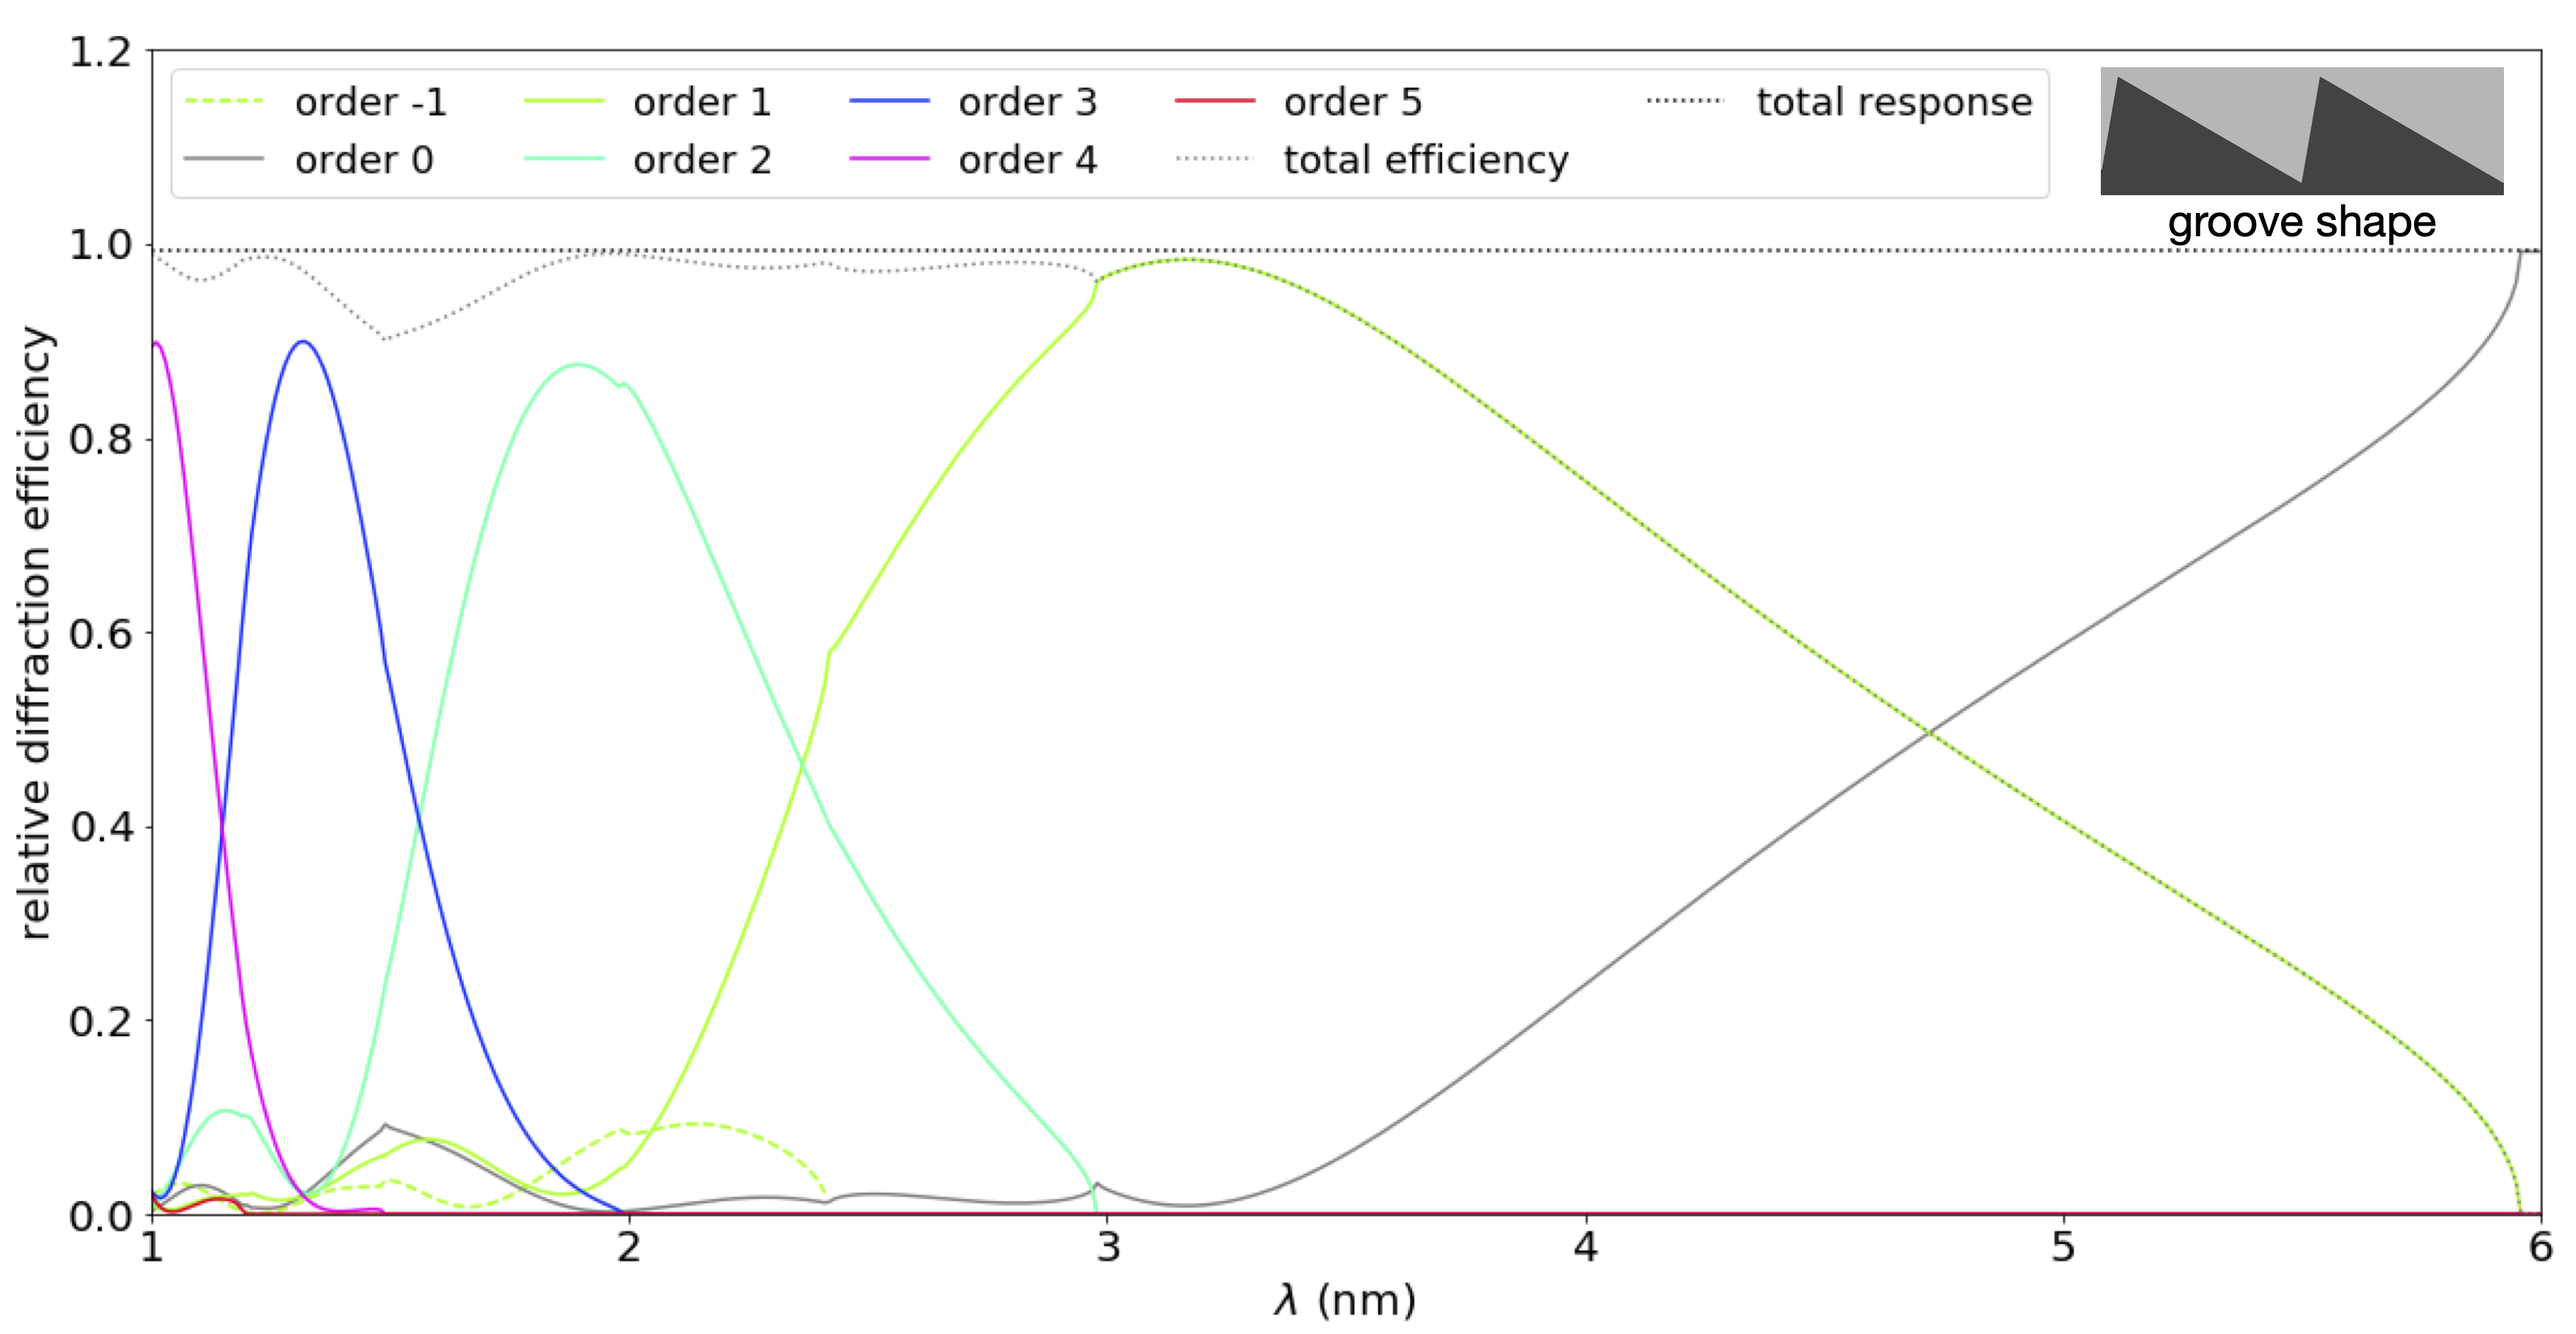
\includegraphics[scale=0.23]{Chapter-2/Figures/perf_ex.png}
 \caption[Example of predicted diffraction efficiency from a perfectly conducting grating using \textsc{PCGrate-SX}]{Example of predicted diffraction efficiency from a perfectly conducting grating emulated using $\tilde{\nu} (\omega) = \num{10000} (1+ i)$ for a border index of refraction in \textsc{PCGrate-SX} (v.\ 6.1) under \emph{perfect conductivity mode}. With the total response of the grating, $\mathscr{E}_{\text{tot}} + \mathscr{E}_0$, approaching unity, $\mathscr{E}_n$ is here interpreted as relative efficiency such that reflectivity must be taken into account separately [\emph{cf.\@} \cref{fig:pcgrate_example_au}].}\label{fig:pcgrate_example_perf}
 \end{figure}
An example of this is shown in \cref{fig:pcgrate_example_perf}, where, as indicated in the figure inset, the grating profile is assumed to be triangular with a $\delta = 30^{\circ}$ active blaze angle and an $80^{\circ}$ opposite angle to yield a groove depth of $h \lessapprox \SI{85}{\nm}$ at $d = \SI{160}{\nm}$. 
Meanwhile, a plane wave of radiation with $\SI{1}{\nm} \leq \lambda \leq \SI{5}{\nm}$ is taken to be incident with a polar angle of $\alpha = 25^{\circ}$ and a half-cone opening angle of $\gamma = 1.5^{\circ}$ to yield propagating orders with $n$ ranging from \numrange{-1}{5}. 
The diffraction efficiency, $\mathscr{E}_n$, for each order is shown as a colored curve, where each maximum corresponds to the blaze wavelength in each propagating order.\footnote{Note that the locations of these maxima may differ from what is predicted by \cref{eq:blaze_wavelength,eq:blaze_wavelength_general} for the blaze wavelength. This is a symptom of the scalar treatment of gratings [\emph{cf.\@} \cref{ap:grating_basics}] being insufficient for modeling the efficiency of x-ray reflection gratings accurately.} 
Moreover, the total diffraction efficiency, $\mathscr{E}_{\text{tot}} \equiv \sum_{n \neq 0} \mathscr{E}_n$, and the total response, $\mathscr{E}_{\text{tot}} + \mathscr{E}_0$, are shown as gray and black dotted lines, respectively. 
Because $\mathscr{E}_{\text{tot}}$ here approaches unity, $\mathscr{E}_n$ can be taken to represent relative efficiency. 

\subsection{Accounting for Soft X-ray Reflectivity}\label{sec:refl_account} 
%%%%%%%%%%%%%%%%%%%%%%%%%%%%%%%%%%%%%%%%%-------------------------------------------------
As a result of the integral method for a perfectly-conducting grating interface effectively giving relative efficiency [\emph{cf.\@} \cref{sec:grat_bound_consider}], reflectivity must be taken into account separately to predict absolute efficiency. 
For an ideal blazed grating, this can be treated by multiplying the predicted relative efficiency by an expression for specular reflectivity, $\mathcal{R}$, from the surface of the groove facets \cite{antonakakis14}. 
If it can be assumed that only one side of the groove facets is illuminated\footnote{This is often the case for a near-Littrow configuration defined by $\alpha \approx \delta$, where $\alpha$ is the azimuthal incidence angle and $\delta$ is the blaze angle. However, this approximation may break down for values of $\alpha$ considerably smaller than $\delta$ or for topographies with a relatively shallow opposite angle. Nonetheless, \textsc{PCGrate-SX} takes into account reflectivity for any grating profile.} and that surface roughness is negligible [\emph{cf.\@} \cref{sec:rough_surface}], this can be written as 
\begin{equation}\label{eq:absolute_eff_approx}
 \mathscr{E}_n \to \mathscr{E}_n \mathcal{R}_F (\zeta) = \underbrace{\frac{\cos \left( \beta \right)}{\cos \left( \alpha \right)} \norm{\tilde{r}^{(n)}}^2}_{\text{\cref{eq:rel_efficiency}}} \mathcal{R}_F (\zeta) ,
 \end{equation}
where $\tilde{r}^{(n)} \equiv \mathcal{A}_n'' / \mathcal{A}_0$ and $\mathcal{R}_F (\zeta)$ is Fresnel reflectivity at a grazing-incidence angle $\zeta$ [\emph{cf.\@} \cref{eq:fresnel_refl_def}].\footnote{Relative to the groove-facet plane defined by a blaze angle $\delta$, this incidence angle is given by \cref{eq:angle_on_groove} [\emph{cf.\@} \cref{fig:conical_reflection_edit}].} 
Because reflectivity is virtually polarization insensitive for grazing-incidence soft x-rays [\emph{cf.\@} \cref{sec:reflectivity_polarization}], $\mathcal{R}_F (\zeta)$ can be taken to represent Fresnel reflectivity in s-polarization, given for a thick slab by \cref{eq:s_reflectivity}. 

To illustrate the validity of \cref{eq:absolute_eff_approx}, the \textsc{PCGrate-SX} model from \cref{fig:pcgrate_example_perf} is reproduced in \cref{fig:pcgrate_example_au} for a gold interface. 
\begin{figure}
 \centering
 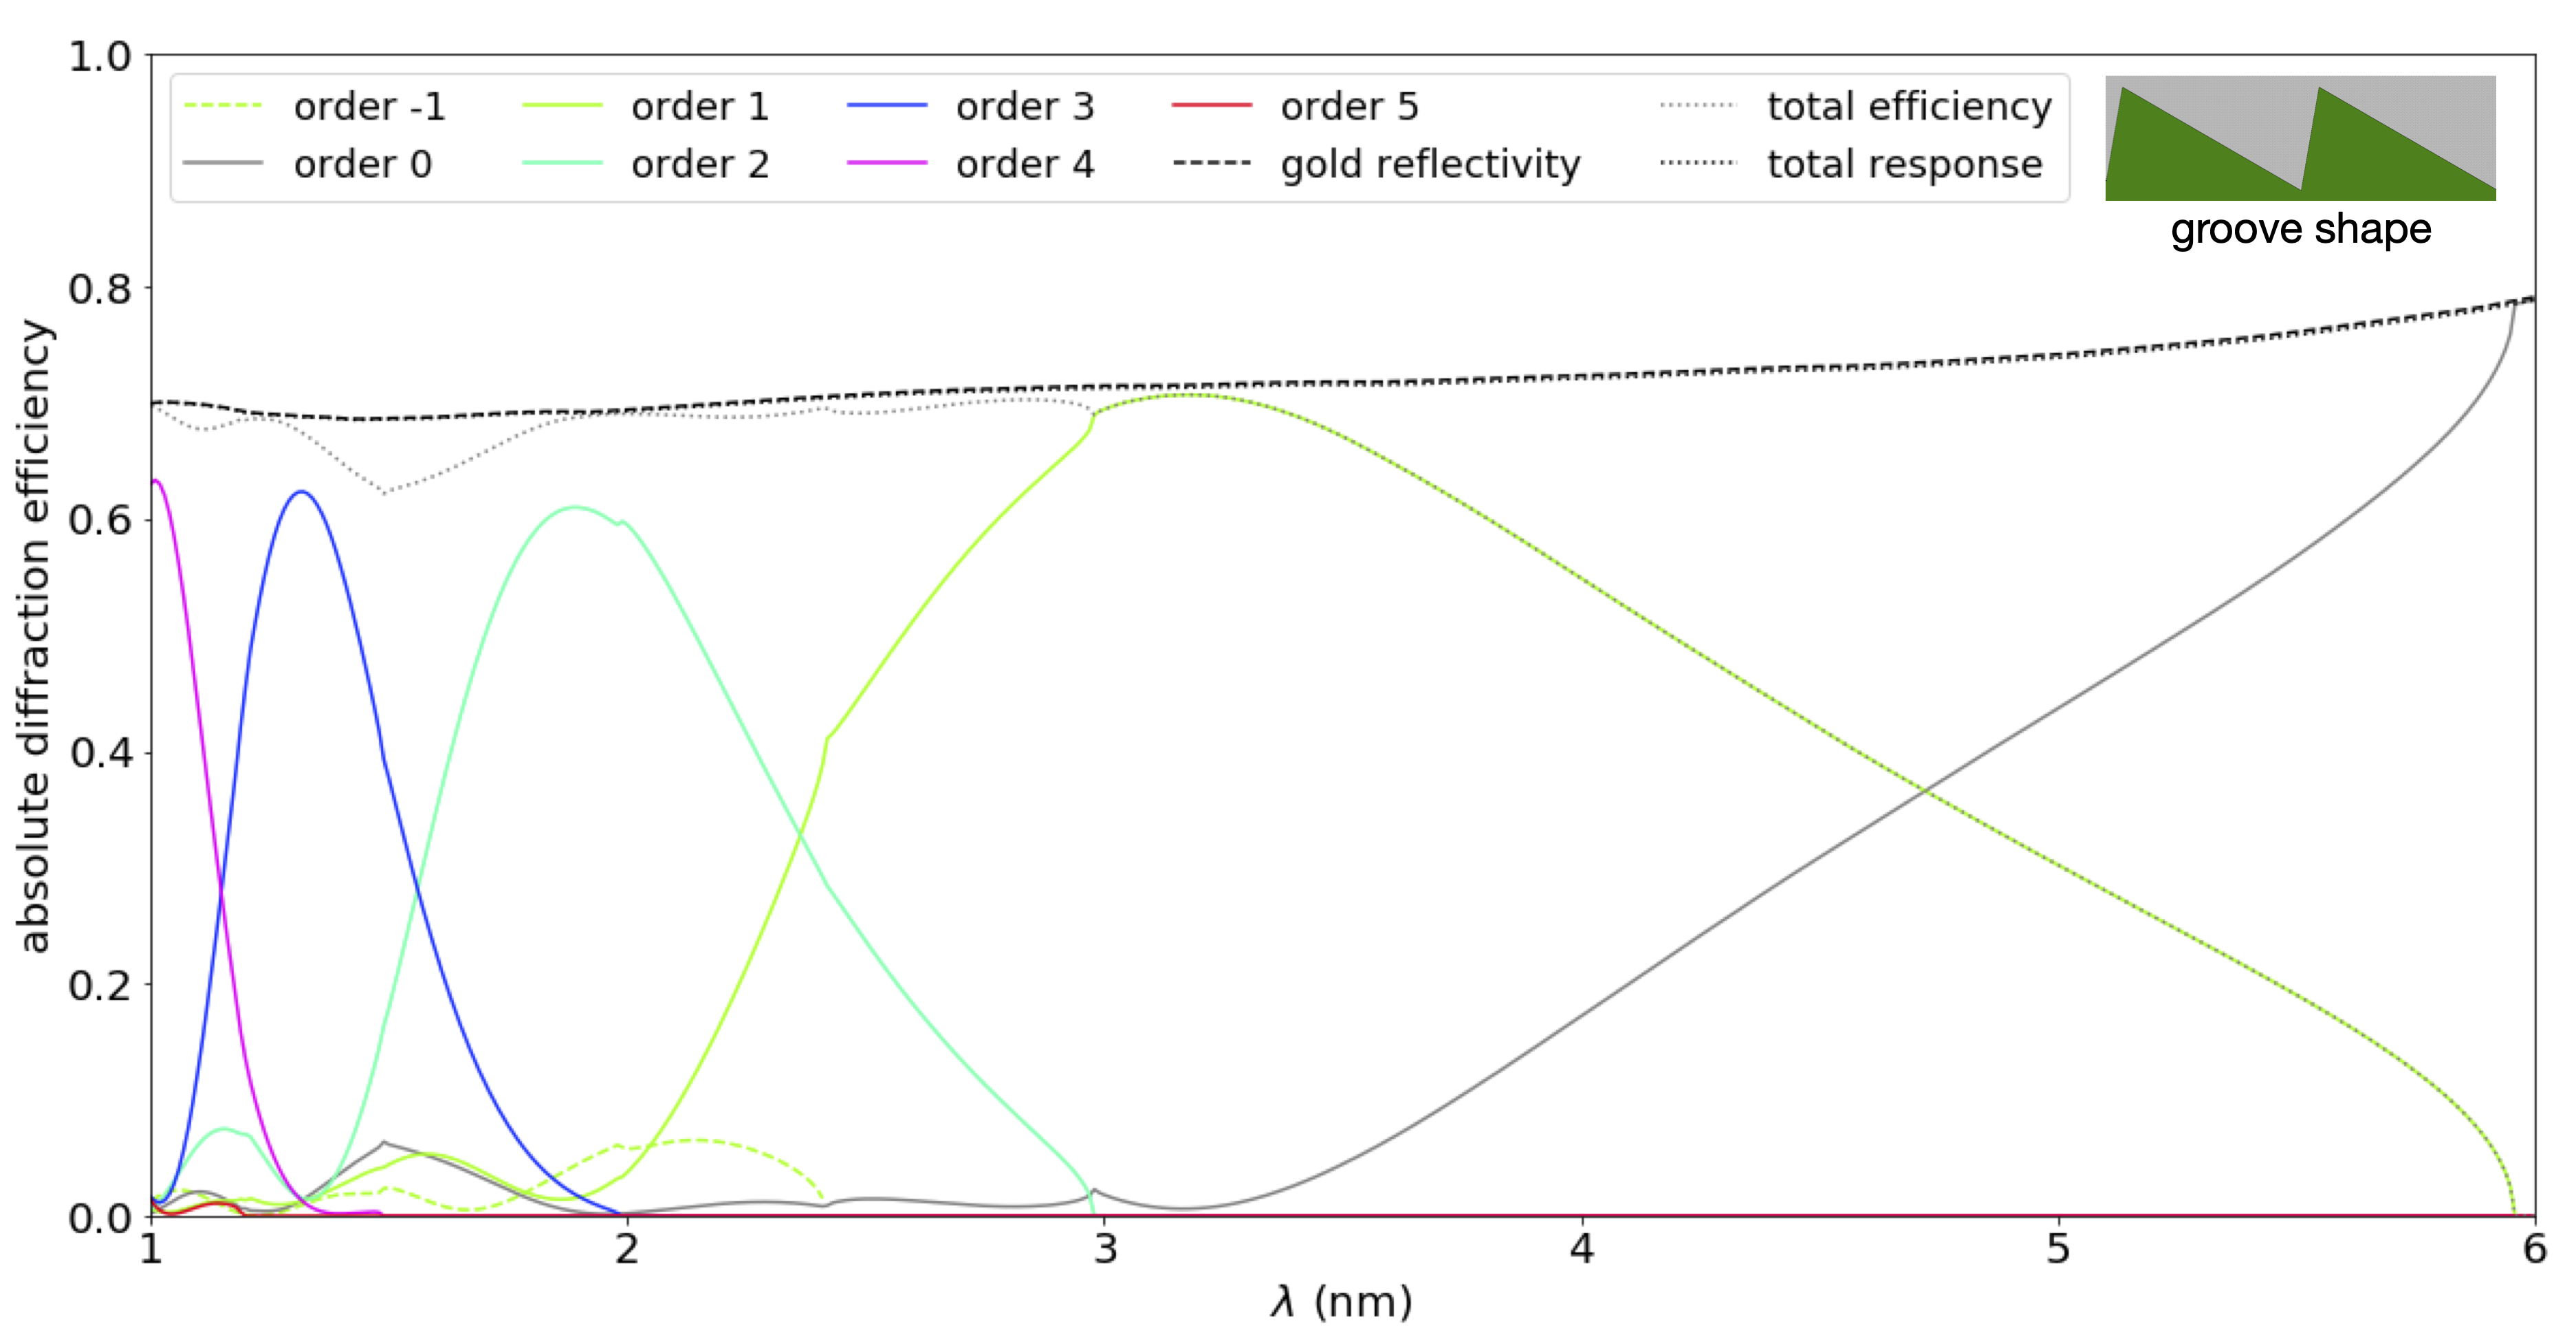
\includegraphics[scale=0.23]{Chapter-2/Figures/au_ex.png}
 \caption[Example of predicted diffraction efficiency for a gold grating using \textsc{PCGrate-SX} under perfect conductivity mode]{Example of predicted diffraction efficiency for a gold grating using \textsc{PCGrate-SX} (v.\ 6.1) under perfect conductivity mode using the same parameters as \cref{fig:pcgrate_example_perf}. The total response of the grating predicted by \textsc{PCGrate-SX} very closely matches Fresnel reflectivity of an equivalent surface at a grazing incidence angle $\zeta \equiv \arcsin \left[ \sin \left( \gamma \right) \cos \left( \delta - \alpha \right) \right]$ [\emph{cf.\@} \cref{eq:angle_on_groove}].}\label{fig:pcgrate_example_au}
 \end{figure}
That is, using data for $\tilde{\nu} (\omega)$ from \cref{fig:X-ray_index}, which were obtained from the CXRO online database \cite{CXRO_database} assuming standard density, \textsc{PCGrate-SX} modulates $\mathscr{E}_n$ predicted for a perfectly conducting grating by the Fresnel reflectivity of a gold slab, which can be taken to represent an overcoat with a thickness several times larger than the penetration depth, $\mathcal{D}_{\perp}$ [\emph{cf.\@} \cref{eq:penetration_depth}].  
In \cref{fig:pcgrate_example_au}, the total response predicted by \textsc{PCGrate-SX} matches $\mathcal{R}_F (\zeta)$ for $\zeta \approx 1.49^{\circ}$, which is determined from $\zeta \equiv \arcsin \left[ \sin \left( \gamma \right) \cos \left( \delta - \alpha \right) \right]$ using $\gamma = 1.5^{\circ}$ and $\abs{\delta - \alpha} = 5^{\circ}$ [\emph{cf.\@} \cref{eq:angle_on_groove}]. 
This indicates that the sum of propagating orders is equal to the Fresnel reflectivity of an equivalent surface:
\begin{equation}
 \sum_{n}^{\text{prop.}} \mathscr{E}_n = \mathcal{R}_F , 
 \end{equation}
which is expected from \cref{eq:absolute_eff_approx}. 
While this relation can be shown more rigorously by solving the Helmholtz equation for a grating border with finite conductivity \cite{Goray10}, this method of predicting absolute diffraction is often sufficient for modeling the behavior of x-ray reflection gratings \cite{Marlowe16}. 

The effect of surface roughness on groove facets can be treated in a similar manner to the scenario of rough mirror flat [\emph{cf.\@} \cref{sec:rough_surface}]. % described in \cref{sec:rough_surface}. 
For the special case of an isotropic, normally-distributed rough surface with a small \emph{root mean square (RMS) roughness} $\sigma$ and a \emph{correlation length} $\ell_{\text{corr}}$ [\emph{cf.\@} \cref{eq:surface_variance,eq:auto_correlation_normal}], $\mathcal{R}_F$ is damped by an exponential factor in the limit of either small or large $\ell_{\text{corr}}$. 
That is, for $\abs{k_{\perp}} \sigma \ll 1$, where $k_{\perp} \equiv - k_0 \sin \left( \zeta \right)$ is the component of $\mathbold{k}$ perpendicular to the groove facet, the \emph{Nevot-Croce factor} derived in appendix~\ref{sec:NC_factor} is valid for small $\ell_{\text{corr}}$ such that $\ell_{\text{corr}} k_{\perp}^2 \ll k_0$ \cite{deBoer95}. 
With the typical size of rough features being too small to produce a diffraction pattern, this quantity describes the fraction of specularly reflected radiation lost due to absorption. % as described in appendix~\ref{sec:NC_factor}. 
For a reflective overcoat that can be treated as a thick slab, the Nevot-Croce factor can be used to modify Fresnel reflectivity [\emph{cf.\@} \cref{eq:NC_refl_ratio}]:
\begin{equation}
 \mathcal{R}_F \to \mathcal{R}_F \norm{\mathrm{e}^{- 2 k_{\perp} \tilde{k_{\perp}}' \sigma^2}}^2 = \mathcal{R}_F \mathrm{e}^{-4 k_0^2 \sin \left( \zeta \right) \Re \left[ \sqrt{\tilde{\nu}^2 (\omega) - \cos^2 \left( \zeta \right) } \right] \sigma^2} ,
 \end{equation}
where $\tilde{k_{\perp}}' = - k_0 \sqrt{\tilde{\nu}^2 (\omega) - \cos^2 \left( \zeta \right)}$ is the component of $\mathbold{\tilde{k}}'$ perpendicular to the groove facet. 
Depending on $\zeta$ and $\lambda$, this Nevot-Croce factor serves an an approximate treatment for groove facets that are dominated by very small lateral surface features. 

Diffuse scattering from facet surface roughness is expected to occur in situations where $\ell_{\text{corr}}$ takes on a value too large to justify use of the Nevot-Croce factor. 
While treating such a scenario rigorously requires using an integral method similar to that described in \cref{sec:grat_bound_consider} \cite{Daillant2009}, a single mode of surface roughness can be treated as a sinusoidal diffraction grating with the effective \emph{surface wavelength}, $\Lambda$, replacing $d$, [\emph{cf.\@} appendix~\ref{sec:intermediate_rough}]. 
Relative to the groove-facet plane, the resulting diffraction pattern has in-plane scattering dominating over off-plane scattering by a factor of $\zeta^{-1}$ [\emph{cf.\@} \cref{fig:in_plane_scatter,fig:off_plane_scatter,eq:in-plane_scatter_angle,eq:off-plane_scatter_angle}]. 
In the limit of very large $\ell_{\text{corr}}$, the \emph{Debye-Waller factor} derived in appendix~\ref{sec:DW_factor} [\emph{cf.\@} \cref{eq:DW_refl_s,eq:DW_factor}] is valid for modeling a reduction in $\mathcal{R}_F$ due to surface roughness: 
\begin{equation}
 \mathcal{R}_F \to \mathcal{R}_F \abs{\mathrm{e}^{-2 k_{\perp}^2 \sigma^2}}^2 = \mathcal{R}_F \mathrm{e}^{-4 k_0^2 \sin^2 \left( \zeta \right) \sigma^2} .
 \end{equation}
A similar factor can be formulated for line-edge and roughness in laminar gratings but its applicability to blazed gratings is limited and not used in this dissertation \cite{Fernandez19,McCurdy20}. 

\section{Summary}\label{sec:ch2_summary} 
%%%%%%%%%%%%%%%%%%%%%%%%%%%%%%%%%%%%%%%%%-------------------------------------------------
The spectral sensitivity of an x-ray grating spectrometer such as the \emph{XGS}, in addition to spectral resolving power, hinges on the instrumental collecting area, which depends directly on the absolute diffraction efficiency of individual reflection gratings used in an extreme off-plane, near-Littrow configuration with $\alpha \approx \delta$ and $\zeta \lessapprox \gamma$ [\emph{cf.\@} \cref{ch:introduction}]. 
As described in \cref{sec:als_testing}, this quantity can be measured in the EUV and soft x-ray at beamline 6.3.2 of the ALS \cite{ALS_632,Underwood96,Gullikson01} by measuring the intensity of the diffracted beam for each propagating order relative to the incident beam after establishing a desired grating geometry using stage rotations and in-situ analysis of the diffracted arc \cite{Miles18}. 
Measured results can be modeled using the \textsc{PCGrate-SX} software package, which employs the integral method for Green's functions to solve the Helmholtz equation for a user-defined grating boundary [\emph{cf.\@} \cref{sec:integral_method}].  
This boundary value problem can be simplified with the assumption of a perfectly-conducting grating boundary and polarization insensitivity, which has been justified experimentally \cite{Marlowe16}. 
When taking into account Fresnel reflectivity for blazed groove facets, the effect of surface roughness can be treated in certain limiting cases. 
The methodology described in this chapter for taking measurements at the beamline and modeling the gathered data using \textsc{PCGrate-SX} is utilized for the experiments described in \cref{ch:master_fab,ch:grating_replication}.